\documentclass[journal]{IEEEtran}

% *** GRAPHICS RELATED PACKAGES ***
%
\ifCLASSINFOpdf
  % \usepackage[pdftex]{graphicx}
  % declare the path(s) where your graphic files are
  % \graphicspath{{../pdf/}{../jpeg/}}
  % and their extensions so you won't have to specify these with
  % every instance of \includegraphics
  % \DeclareGraphicsExtensions{.pdf,.jpeg,.png}
\else
  % or other class option (dvipsone, dvipdf, if not using dvips). graphicx
  % will default to the driver specified in the system graphics.cfg if no
  % driver is specified.
  % \usepackage[dvips]{graphicx}
  % declare the path(s) where your graphic files are
  % \graphicspath{{../eps/}}
  % and their extensions so you won't have to specify these with
  % every instance of \includegraphics
  % \DeclareGraphicsExtensions{.eps}
\fi
% graphicx was written by David Carlisle and Sebastian Rahtz. It is
% required if you want graphics, photos, etc. graphicx.sty is already
% installed on most LaTeX systems. The latest version and documentation
% can be obtained at: 
% http://www.ctan.org/tex-archive/macros/latex/required/graphics/
% Another good source of documentation is "Using Imported Graphics in
% LaTeX2e" by Keith Reckdahl which can be found at:
% http://www.ctan.org/tex-archive/info/epslatex/
%
% latex, and pdflatex in dvi mode, support graphics in encapsulated
% postscript (.eps) format. pdflatex in pdf mode supports graphics
% in .pdf, .jpeg, .png and .mps (metapost) formats. Users should ensure
% that all non-photo figures use a vector format (.eps, .pdf, .mps) and
% not a bitmapped formats (.jpeg, .png). IEEE frowns on bitmapped formats
% which can result in "jaggedy"/blurry rendering of lines and letters as
% well as large increases in file sizes.
%
% You can find documentation about the pdfTeX application at:
% http://www.tug.org/applications/pdfte

% correct bad hyphenation here
\hyphenation{op-tical net-works semi-conduc-tor}

\usepackage{graphicx}
\usepackage{amsmath}
\usepackage{amssymb}
\usepackage{color}
\usepackage{epsfig}
\usepackage{tabularx}
\usepackage{ctable}
\usepackage{multirow}
\usepackage{subfigure}
\usepackage{mathrsfs}
\usepackage{mathtools}
\usepackage{hyperref}
\usepackage{algorithm}
\usepackage{algpseudocode}
\usepackage{booktabs}
% gray scaled table
%\newcommand\gray{gray}
%
%\newcommand\ColCell[1]{%
  %\pgfmathparse{#1<.6?1:0}%
    %\ifnum\pgfmathresult=0\relax\color{white}\fi
  %\pgfmathparse{1-#1}%
  %\expandafter\cellcolor\expandafter[%
    %\expandafter\gray\expandafter]\expandafter{\pgfmathresult}#1}
%
%\newcolumntype{E}{>{\collectcell\ColCell}c<{\endcollectcell}}


% format argmin
\DeclareMathOperator*{\argmin}{arg\,min}

% algorithm title
%\makeatletter
%\def\BState{\State\hskip-\ALG@thistlm}
%\makeatother





\begin{document}
%
% paper title
% can use linebreaks \\ within to get better formatting as desired
% Do not put math or special symbols in the title.
\title{Hahaha Person-Independent Expression Recognition Using Sparse Expression Residual}
%
%
% author names and IEEE memberships
% note positions of commas and nonbreaking spaces ( ~ ) LaTeX will not break
% a structure at a ~ so this keeps an author's name from being broken across
% two lines.
% use \thanks{} to gain access to the first footnote area
% a separate \thanks must be used for each paragraph as LaTeX2e's \thanks
% was not built to handle multiple paragraphs
%

\author{XX,~\IEEEmembership{Member,~IEEE,}
				YY~\IEEEmembership{Member,~IEEE}% <-this % stops a space
\thanks{\IEEEcompsocthanksitem Acknowledgment: \IEEEcompsocthanksitem 

}}


% The paper headers
\markboth{IEEE Transaction on Multimedia,~Vol.~, No.~, }%
{Shell \MakeLowercase{\textit{et al.}}: Bare Demo of
IEEEtran.cls for Computer Society Journals}
% make the title area
\maketitle

% As a general rule, do not put math, special symbols or citations
% in the abstract or keywords.
\begin{abstract}
Person-independent expression recognition aims to recognizing facial expressions of an \textit{unseen} subject from videos. This remains a challenging problem due to that the facial muscle motion for a typical facial expression, which should be similar irrespective of the subject identity, is difficult to be characterized across population. The classifiers can be easily over-fitted to person-specific facial appearances rather than the person-independent muscle motion from expressions. Additionally, the problem becomes even more challenging when the rigid head motion is coupled with non-rigid facial muscle motion in uncontrolled settings. To tackle these challenges, we model an expression video as a combination of two parts: (1) a set of low-rank components that are representative of person-independent expression prototypes, namely Low-rank Expressions (LRE); (2) a set of sparse appearance residuals that capture the muscle motion of individual frames, namely Sparse Expression Residuals (SER). To avoid over-fitting, we explicitly model the person-independent transformation of individual frames to a canonical reference space in the minimization objective. We show that the objective formulation can be simplified and solved by an efficient sparse low-rank recovery algorithm. We then carry out a comparative study of the recently successful Emotion Avatar Images~\cite{Yang_SMCB12} (EAI) models and the proposed LRE representation, qualitatively illustrating the merits of these models in representing expressions in a person-independent manner. We also demonstrate that the SER can further improve the recognition performance, when both static and dynamic texture features are extracted out of SER. Extensive qualitative and quantitative results demonstrate that our approach not only establishes informative visual representations but also yields the state-of-the-art recognition performance.


\end{abstract}

% Note that keywords are not normally used for peerreview papers.
\begin{IEEEkeywords}
person-independent facial expression, low-rank expression, sparse expression residual, Emotion Avatar Image (EAI)
\end{IEEEkeywords}






% For peer review papers, you can put extra information on the cover
% page as needed:
% \ifCLASSOPTIONpeerreview
% \begin{center} \bfseries EDICS Category: 3-BBND \end{center}
% \fi
%
% For peerreview papers, this IEEEtran command inserts a page break and
% creates the second title. It will be ignored for other modes.
\IEEEpeerreviewmaketitle



\section{Introduction}

\IEEEPARstart{A}{ffective} computing have been attracting an increasing amount of attentions from the point of view of psychology and computer science~\cite{Picard03}. As a primary channel of conveying emotion, automatic facial expression analysis has been extensively studied~\cite{Pantic_PAMI00}\cite{Torre11}. Although there have been a rich body of research on facial expression recognition in controlled environments~\cite{Torre11}, a recent expression analysis challenge~\cite{FERA11} indicates that person-independent expression recognition remains a difficult problem in uncontrolled settings, due to the following reasons:

\begin{figure}[htbp]
	\centering
		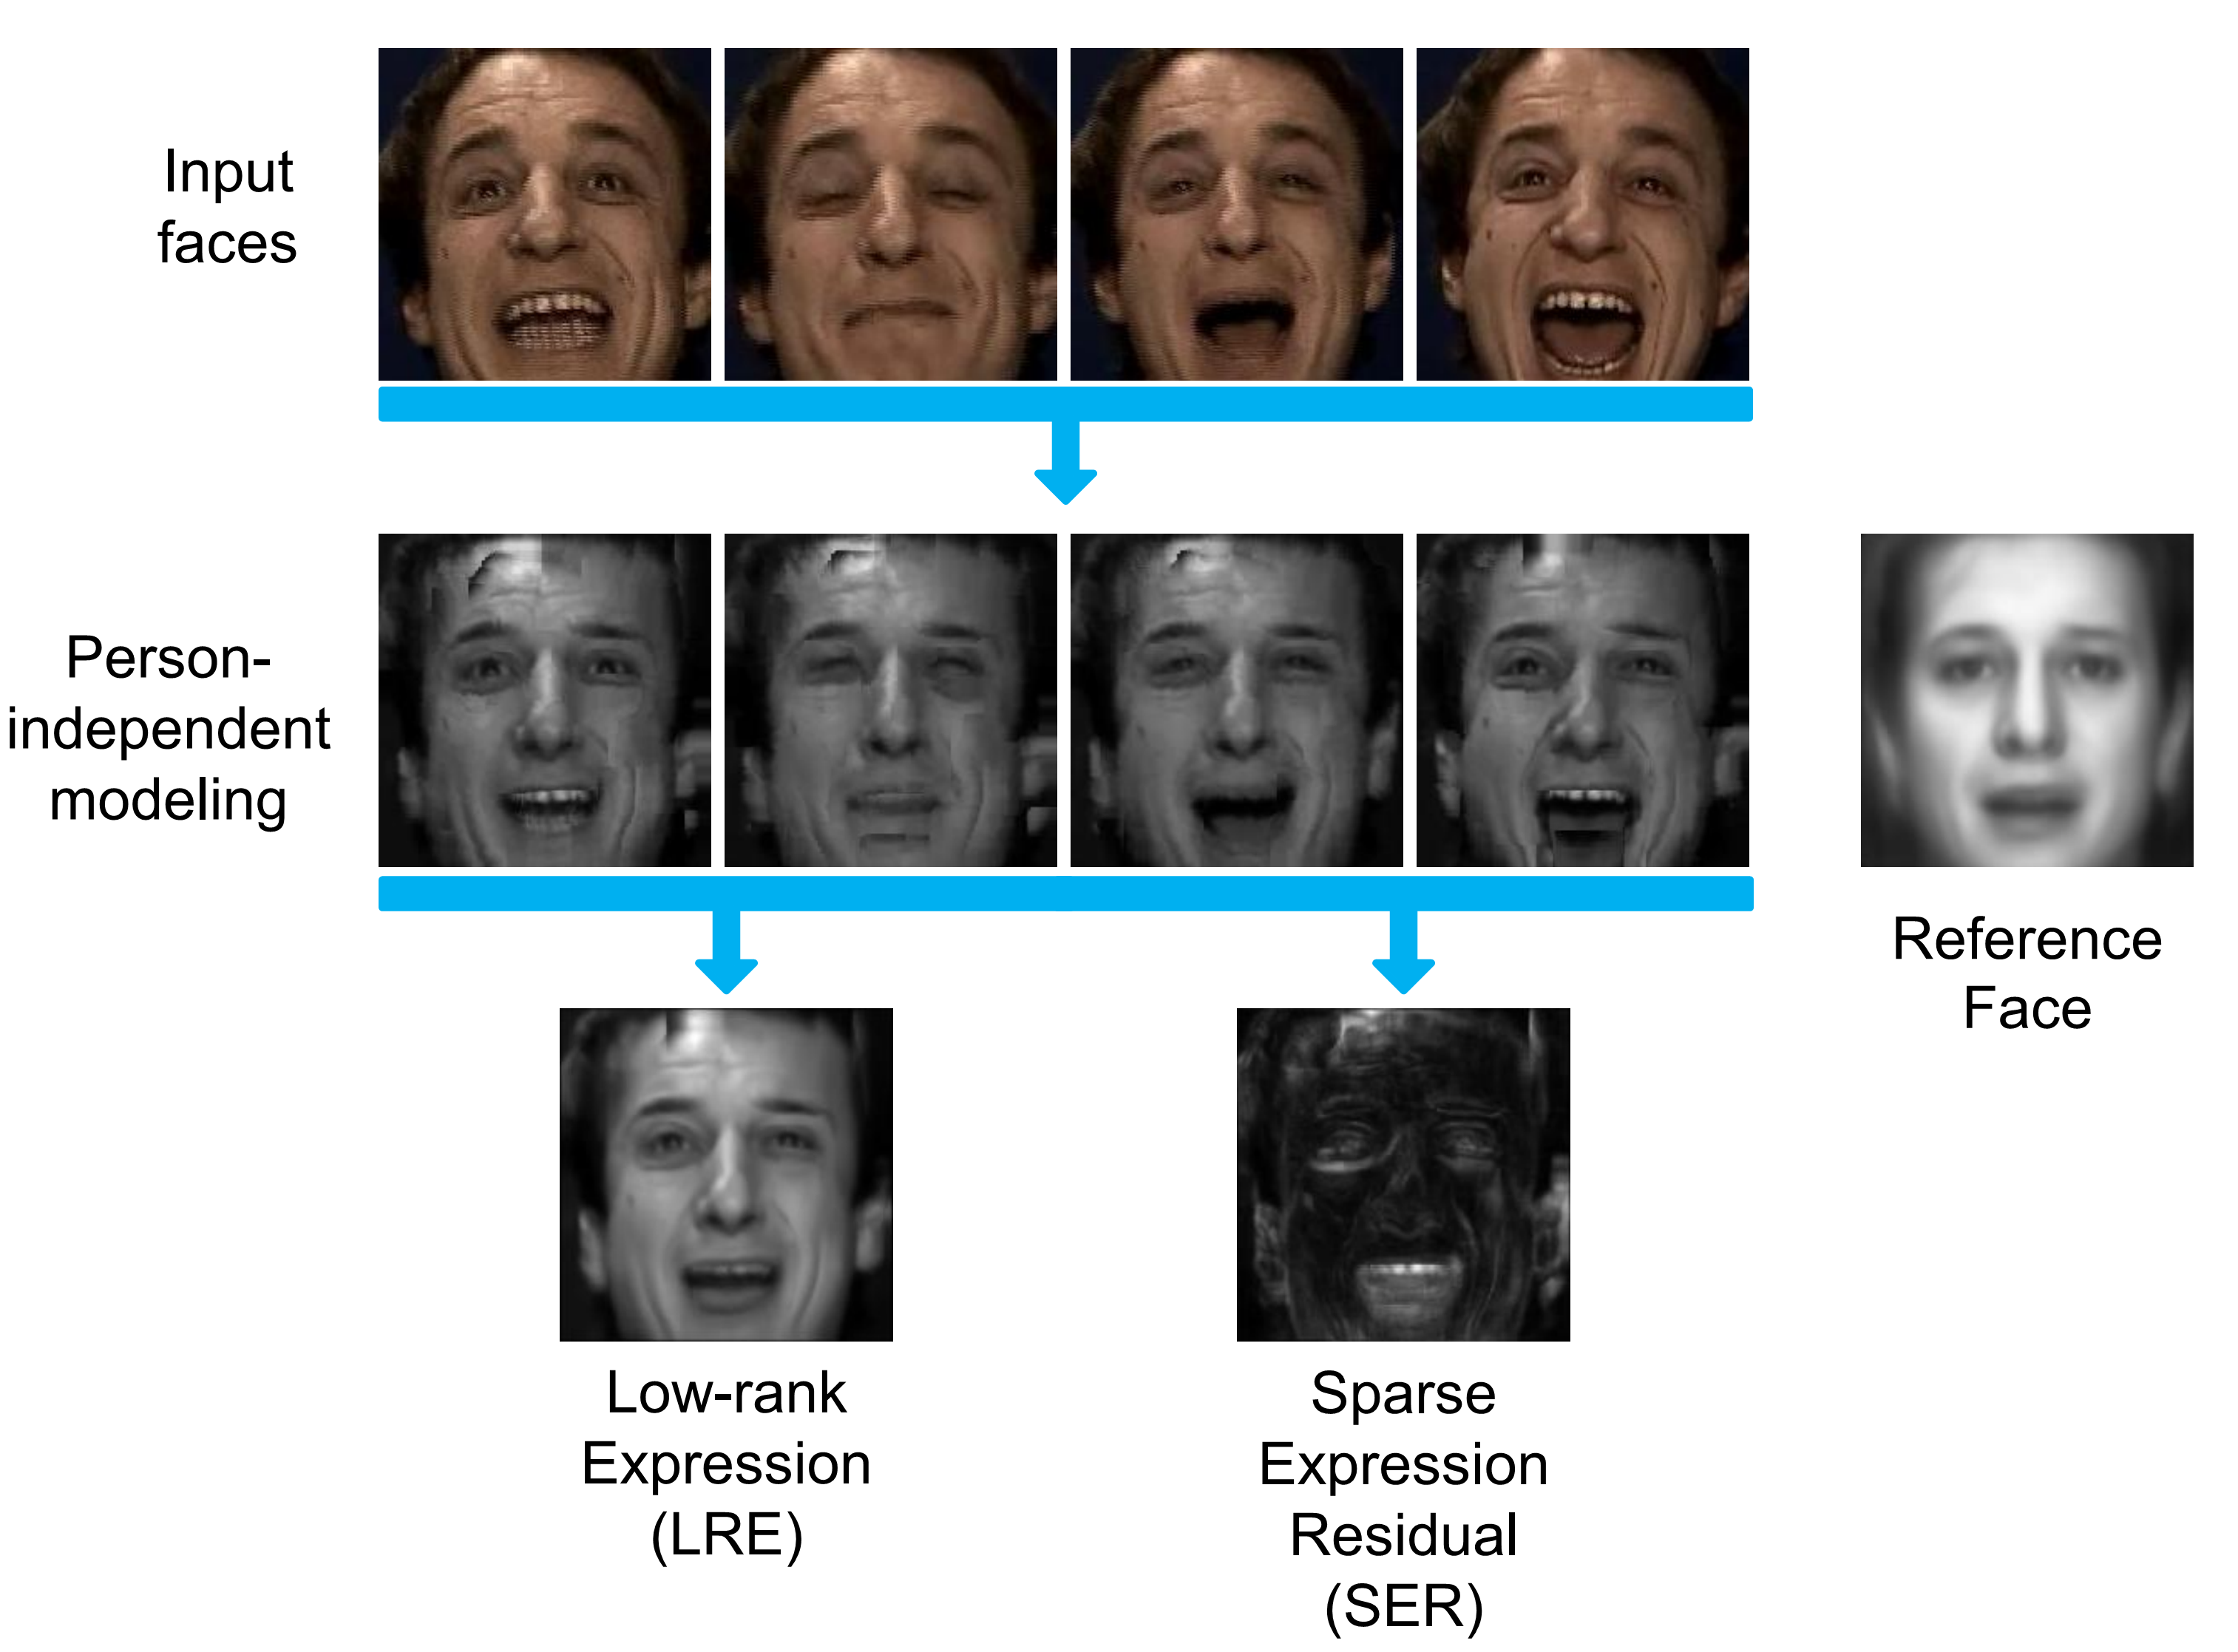
\includegraphics[width=.95\columnwidth]{pics/splash.png}
	\caption{The overview of our approach. We observe that (1) a facial expression sequence possess an inherent \textit{global} model (\textit{e.g.}, lip corner expansion for \textit{Happiness} in this case); and (2) each frame has its own \textit{local} properties (\textit{e.g.}, various muscle motion intensities), which describe the facial dynamics. Due to the face anatomy constraints~\cite{Ekman78}, the muscle motion that characterize the local deformation is sparsely distributed. Inspired by these observations, we model each frame as (1) a low-rank structure that represents the global expression appearance jointly estimated from the entire sequence (\textit{i.e.}, LRE), and (2) an additive sparse residual that represents the deviations from the low-rank structure (\textit{i.e.}, SER). Moreover, the person-independent factor is modeled as a transformation to a canonical space (Reference face), avoiding over-fitting for classification. Both LRE and SER provide viable manners to extract meaningful facial expression dynamics, yielding superior recognition performances. To appreciate the information captured by the LRE and SER representations, the bottom row shows the mean representation of the decomposed sequence. The mean LRE retains the global appearance and the mean SER captures the local motion around mouth and eye areas.}
	\label{fig:splash}
\end{figure}

\begin{enumerate}

\item \textbf{Compound Motion:} the facial expression appearance in video consists of rigid head motion and non-rigid muscle motion. The rigid head motion consists of in-plane and out-of-plane rotations. Aligning 2D faces by rectifying the out-of-plane rotation is considerably more difficult than in-plane rotation due to the 3D shape characteristics of a human face. Most approaches in the literature~\cite{Bartlett_FG11}\cite{Valstar_FERA11} only recover the in-plane rotation by computing an affine transformation based on facial feature correspondences. Further, segmenting the non-rigid muscle motion, which reveals the true facial expression, from the rigid head motion is an inherently challenging problem due to the 2D imaging procedure.

\item \textbf{Person-specific Effect:} in a facial expression recognition task, the goal is to discover robust features to discriminate various expressions. Psychological study~\cite{Fridlund_87} shows, and many vision-based expression analysis rely on~\cite{Pantic_PAMI00}, that there are six basic prototype expressions that have similar properties across various cultures, namely, \textit{Happiness}, \textit{Sadness}, \textit{Surprise}, \textit{Fear}, \textit{Anger}, and \textit{Disgust}. Under this assumption, an desired vision-based expression recognition system should extract features that are cultural-independent or even, person-independent. However, typical facial expression recognition systems~\cite{Bartlett_FG11}\cite{Valstar_SMCB12} uses generic appearance- or geometry-based features to characterize a expression, without modeling the person-independent property. Thus, person-specific features is retained and it is unclear if the classifier is trained to recognize person-independent expressions. This can yields an over-fitted classification model that ultimately degrades the recognition accuracy when testing on unseen subjects. An ``ideal'' expression recognition system is expected to eliminate the entire person-specific information, distilling the person-independent motion solely from expressions. There has been some work~\cite{Yang_SMCB12}\cite{Dahmane_TMM14} that attempt to diminish the person-specific effect, yielding plausible performances. This demonstrate that person-independent modeling is a key issue in generalizing expression recognition systems to unseen subjects.

\end{enumerate}

In this paper, the problem we intend to solve is as follows: given a video sequence of a facial expression (after temporal segmentation), the goal is to classify the this video as one of the categorical expression, such as \textit{Happiness}, \textit{Anger}, etc. 

From a video processing perspective, the approaches can be categorized into three strategies for video-based expression recognition. First, A wide range of methods~\cite{Bartlett_FG11}\cite{Valstar_SMCB12} process each frame individually, where they extract features from each frame and carry out majority voting for the entire sequence. Second, temporal features are used to capture the muscle dynamics of facial expressions~\cite{Zhao_PAMI07}\cite{Huang11}. These approaches typically requires accurate alignment results in order to generate meaningful dynamic features. Third, an entire video is summarized into an image-based representation that captures the expression appearance~\cite{Yang_SMCB12}\cite{Dahmane_TMM14}. This approach completely abandons the dynamic information, and cannot model the temporal characteristic of facial expressions. In essence, the aforementioned strategies summarize the video-based expression data at different resolutions. 

In this work, we depart from all the previous strategies and analyze the facial expression at a finer resolution. We observe that, on one hand, samples of one expression sequence are correlated and possess similar \textit{global} characteristics (\textit{e.g.}, lip corner expansion for \textit{Happiness}); one the other hand, each sample has its own \textit{local} properties (\textit{e.g.}, various muscle motion intensities for different expression stages such as \textit{onset}, \textit{apex}, or \textit{offset}), which could be used to describe facial dynamics. Due to the face anatomy constraints~\cite{Ekman78}, the muscle motion that characterize the local deformation is sparsely distributed. Inspired by these observations, we model each frame as (1) a low-rank structure that represents the global expression appearance jointly estimated from the entire sequence, and (2) an additive sparse residual that represents the deviations from the low-rank structure. As shown in Fig.~\ref{fig:splash}, both static and dynamic features are extracted from the Low-rank Expression (LRE) and the Sparse Expression Residual (SER) representations for expression recognition. In addition, we explicitly model the person-independent facial expression appearance transformation in a low-rank recovery framework. The person-independent factor is modeled as a non-linear transformation function, which can be approximated by matching a target face to a canonical reference face in a structural sense. Concretely, we approximate this non-linearity by the correspondence of two SIFT feature descriptors, namely SIFT-flow~\cite{Liu_PAMI11}. We then show that the person-independent transformation is independent of the low-rank recovery procedure, leading to an efficient algorithm in the pursuit of the sparse low-rank facial expression appearances. 

In what follows, Section~\ref{sec:related} reviews the related work in the literature and presents our contributions. Subsequently, Section~\ref{sec:decompose} details the modeling of expression images as Low-rank Expression (LRE) and Sparse Expression Residual (SER) representations. In particular, in Section~\ref{sec:eai}, we discuss the relationship of LER with the Emotion Avatar Images (EAI), illustrating in both theory and visual results. Section~\ref{sec:exp} demonstrates the effectiveness of LRE+SER modeling via extensive experimental results. Finally, Section~\ref{sec:conclude} concludes the paper.


\section{Related Work and Our Contributions\label{sec:related}}

We first review the related works in the literature for both facial expression recognition and sparse representation, and then highlight our contributions thereafter. 

\subsection{Facial Expression Recognition}

There is a rich body of work in the literature for automatic facial expression analysis. Earlier work have been focused on recognizing expressions from \textit{static} images, where both facial geometry and textures are used for this task~\cite{Pantic_PAMI00}\cite{Essa_PAMI97}\cite{Donato_PAMI99}. These work contribute to the recently expression analysis in videos~\cite{Bartlett_FG11}\cite{Kaliouby_SMC04}\cite{Valstar_FERA11}, where these systems treat frame individually and attempt to recognize facial expression or Action Units~\cite{Ekman78}. The texture features can be described by descriptors such as Haar-like features~\cite{Whitehill_FG06}, Gabor filters~\cite{Lyons_PAMI99}~\cite{Bartlett_FG11}, Local Binary Patterns (LBP)~\cite{Shan_IVC09}~\cite{Jiang_FG11}, Edge Orientation Histogram~\cite{Levi_CVPR04}, Histogram of Oriented Gradients~\cite{Dalal_CVPR05}\cite{Dhall_FERA11}\cite{Dahmane_FERA11}, Local Phase Quantization~\cite{LPQ}.

As pointed out in~\cite{Ekman2005}~\cite{Ambadar05}, facial muscle \textit{dynamics} play an important role in spontaneous expressions. The pioneer work by Yacoob and Davis~\cite{Yacoob_PAMI96} describes the facial dynamics using optical flow. This immediately raises a question that optical flow highly relies on accurate face tracking and alignment. It is assumed in~\cite{Yacoob_PAMI96} that subjects are with controlled frontal head pose, and thus, a simple thresholding procedure can rule out small motion cause by noise or tracking errors. Moreover, this work ignores the facial texture information, which later works find quite successful in characterizing facial dynamics. For example, Zhao and Pietik\"ainen~\cite{Zhao_PAMI07} extend LBP to the temporal space, namely three orthogonal planes (LBP-TOP), by taking into account the co-occurrence of the patterns. It combines appearance and motion together and achieves outstanding performance for facial expression recognition under controlled settings, \textit{e.g.}, the Cohn-Kanade database~\cite{CKplus}. Similarly, more texture descriptors~\cite{LPQ-TOP} can be extended to spatial-temporal settings, yielding a superior performance. The muscle dynamics can also be characterized by the motion of facial landmarks (\textit{e.g.}, eyebrow corner, mouth corner, etc.). Valstar and Pantic~\cite{Valstar_SMCB12} track a set of landmarks over time and infer facial expressions based on the dynamics of landmark. 

Facial dynamics is easier to capture in controlled lab settings~\cite{CKplus}, where subjects are constraint to have limited head motion and exaggerate facial muscle motion for expression. However, in a more realistic and uncontrolled scenario (\textit{e.g.}, FERA dataset~\cite{Valstar_FERA11}), extracting facial dynamics highly relies on accurate landmark tracking and face alignment. The facial expression imagery consists of the ``compound motion'' from the rigid head motion and deformable facial muscle motion. Ideally, the head motion should be corrected to fully characterize the non-rigid muscle motion, which is directly related to the expressions. It is shown in~\cite{Valstar12}\cite{Yang_SMCB12} that without a reliable alignment result, the dynamic feature is even inferior than static features. Therefore, in this work, we establish a framework that aligns expression images under compound motion from region-based correspondences (in contrast to point-based correspondences), which helps to extract dynamical features much more effectively. 


\subsection{Sparse Representation}

Recently, sparse modeling has been successful for problems such as image restoration~\cite{Yang_CVPR08}, face recognition~\cite{Wright_PAMI09}, and human action recognition~\cite{Qiu_ICCV11}. In particular, sparse representation combined with low-rank modeling can be used to describe robust features directly from an image as a matrix, such as the transform invariant low-rank textures~\cite{Zhang_IJCV12}, group alignment by sparse and low-rank decomposition~\cite{Peng_PAMI12}. In the facial expression related domain,~\cite{Lin12} jointly recovers a dictionary and a set of sparse coefficients to efficiently synthesize 3-D facial expressions.~\cite{Tariq12} learns the mid-level features by sparse coding technique for multi-view expression recognition. It uses sparse codes of local descriptors (such as SIFT) to build features for expression recognition. In contrast, we focus on recovering 2D representations that are of low-rank property for a better (static and/or dynamic) feature extraction. 

\subsection{Our Contributions}
The contributions of this work are the follows:
\begin{enumerate}
\item We observe that each frame of a prototype expression sequence is correlated and consists of a global and a local component. We then propose to model the generic person-independent facial expressions video in a sparse low-rank recovery framework. The sequence is decomposed into two components, termed Low-rank Expression (LRE) and Sparse Expression Residual (SER), which help to extract dynamical facial features more effectively. 

\item We show that a special case of person-independent transformation, via SIFT-flow, results in a low-rank expression model, which visually resembles the successful Emotion Avatar Image (EAI) representations~\cite{Yang_SMCB12} for superior recognition performance for unseen data.

\item We demonstrate that the non-rigid muscle motion captured by the sparse residual component, SER, is an effective representation to extract dynamics from and can further improve the recognition performance. Both quantitative and qualitative evaluations are carried out to justify the improvement. 

\end{enumerate}

\section{Person-independent Expression Modeling\label{sec:decompose}}

\subsection{The Generalized Model} 
We assume that a video is temporally segmented such that it can be described by one labeled category, \textit{e.g.}, prototype expressions (\textit{Happiness} or \textit{Anger}) or Action Units. We then seek to decompose each frame of the sequence into two representations: (1) a low-rank model represents the global appearance of the sequence; (2) a sparse component that characterizes the non-rigid muscle motion for each frame. Formally, given a sequence of faces, we denote $I_1, \ldots, I_n$ as $n$ image observations of a sequence, then

\begin{equation}
I_i = I^{0}_i + e_i,\quad i = 1\cdots n
\end{equation}

\noindent where sparse residual is modeled by an additive term $e_i$, $I^{0}_i$ is the difference between $I_i$ and $e_i$. Further, we denote $v\in\mathscr{R}^{m\times 1}$ to be the vectorized observation $I$. Stacking multiple such vectors results in an observation matrix

\begin{equation}
D = [v_1 | \cdots | v_n] = A + E
\end{equation}

\noindent where $D\in\mathscr{R}^{m\times n}$; $A = [v^{0}_{1} | \cdots | v^{0}_{n}]$ is a low-rank matrix that models the representative structure of an facial expression sequence; $E = [e_{1} | \cdots | e_{n}]$ is a sparse matrix with large magnitude deviations that models the motion of the sequence. Thus, the problem that we try to solve is

\begin{equation} \label{eq:org}
\argmin_{A,E} rank(A)+\gamma \|E\|_0  \quad s.t. \quad D = A + E 
\end{equation}

\noindent where $\|\cdot\|_0$ is the $L_0$ norm which represents the number of non-zero entries in the error term $E$. $\gamma$ is the scaling parameter which controls a weight preference of the rank of $A$ and sparsity of $E$. Although Eq.~\ref{eq:org} is an intuitive formulation, it is intractable in practice due to the non-convexity and discontinuity of rank computation and $L_0$ norm, and the highly non-linearity of the equality constraint. As suggested by many work in sparse low-rank recovery~\cite{Candes11,Lin09,Peng_CVPR10}, this problem can be relaxed by its convex surrogate

\begin{equation} \label{eq:rpca}
\argmin_{A,E} \|A\|_*+\gamma \|E\|_1  \quad s.t. \quad D = A + E 
\end{equation}

\noindent where $\|\cdot\|_*$ is the nuclear norm that captures the sum of all singular values of $A$, \textit{i.e.}, $\|A\|_*=\sum^m_{i=1}\sigma_i(A)$; $\|E\|_1=\sum_{ij}|E_{ij}|$ is the $L_1$ norm of $E$. This new objective is now continuous and convex. 


\subsection{Reference-based Person-Independent Transformation} 

Since a face in each frame, $I_i$, contains pose and identity variations, we intend to carry out the expression recognition task in a canonical space. Specifically, we model the person-independent factor by mapping each face to a reference face model, $I_r$. This strategy has been demonstrated effective in expression recognition particularly in predicting expressions from unseen subjects~\cite{Yang_SMCB12,Dahmane_TMM14}. We model the mapping by a transformation function on the image observation, $D$. Thus, the objective is written as

\begin{equation} \label{eq:rpca}
\argmin_{A,E} \|A\|_*+\gamma \|E\|_1  \quad s.t. \quad \phi (D) = A + E, 
\end{equation}

Here, $\phi (D)$ is defined as a generic function that transforms each face, $I_i$,  in $D$ to the canonical space. One instantiation of the non-linear mapping, which we opt to use in this work, is the structural matching technique, namely, SIFT-flow. 

SIFT flow~\cite{Liu_PAMI11} was originally designed to align an image to its plausible nearest neighbor which can have large variations. It robustly matches dense structural SIFT features between two images, while maintaining spatial discontinuities. The SIFT~\cite{Lowe_ICCV99} feature is first extracted in a pixel-wise fashion. For every pixel in an image, the neighborhood (\textit{e.g.}, $16\times16$) is divided into a $4\times4$ cell array. The orientation of each cell is quantized into 8 bins, generating a $4\times4\times8=128$-dimension vector as the SIFT representation for a pixel, or the so called SIFT image. Subsequently, a dense correspondence is established to match the two SIFT images. Similar to optical flow, the objective energy function is designed as:
\begin{align}
	\label{data_term}
	E(\textbf{w})=&\sum_\textbf{p} min(\left\|s_1 (\textbf{p})-s_2 (\textbf{p}+\textbf{w}(\textbf{p}))\right\|_1 ,t)+
\\\label{small_constraint}
&\sum_\textbf{p} \eta(\left|u(\textbf{p})\right|+\left|v(\textbf{p})\right|) +
\\\nonumber
&\sum_{(\textbf{p},\textbf{q})\in\varepsilon} min(\alpha\left|u(\textbf{p})-u(\textbf{q})\right|,d)+
\\\label{smooth_constraint}
&~~~min(\alpha\left|v(\textbf{p})-v(\textbf{q})\right|,d)
\end{align}

\noindent where $\textbf{p}=(x,y)$ is the grid coordinates of the images, and $\textbf{w}(\textbf{p})=(u(\textbf{p}),v(\textbf{p}))$ is the flow vector at $\textbf{p}$. $u(\textbf{p}),v(\textbf{p})$ are the flow vectors for $x$ direction and $y$ direction respectively. $s_1$ and $s_2$ are two SIFT images to be matched. $\varepsilon$ contains all the spatial neighbors (a four-neighbor system is used). The \emph{data term} in (\ref{data_term}) is a SIFT descriptor match constraint that enforces the match along the flow vector $\textbf{w}(\textbf{p})$. The \emph{small displacement constraint} in (\ref{small_constraint}) allows the flow vector to be as small as possible when no other information is available. The \emph{smoothness constraint} in (\ref{smooth_constraint}) takes care of the similarity of flow vectors for adjacent pixels. In this objective function, the truncated $L1$ norm is used in both the data term and the smoothness term with $t$ and $d$ as the thresholds for matching outliers and flow discontinuities, respectively. $\eta$ and $\alpha$ are weight parameters for the small displacement and smoothness constraint, respectively. The dual-layer loopy belief propagation is used in additional to the coarse-to-fine flow matching scheme to optimize the objective function efficiently.

\begin{figure}[htbp]
	\centering
		\includegraphics[width=\columnwidth]{pics/sift_flow_visual.png}
	\caption{Reference-based alignment via SIFT flow~\cite{Liu_PAMI11} warping. The Avatar Reference is a canonical representation following the work in~\cite{Yang_SMCB12}. The head rotation is corrected and person-specific information is attenuated in both sequence.}
	\label{fig:sift_flow_visual}
\end{figure}


Fig.~\ref{fig:sift_flow_visual} shows SIFT flow warping of faces with respect to AR. Faces in each frame is extracted from Viola-Jones face detector~\cite{Viola_IJCV04}. The reference face images is chosen to be the level-1 Avatar Reference (AR) image~\cite{Yang_SMCB12} generated from the FERA-GEMEP dataset~\cite{Valstar_FERA11}. AR is essentially a face model reflects the expression and identity of the entire population in the dataset. It is computed by an iteratively algorithm that estimates the reference model and the individual expression model simultaneously. It is computed offline and has been demonstrated to perform well across datasets~\cite{Yang_SMCB12}. 

Since we transform each frame to the same reference model, facial features for the entire sequence are coarsely aligned. It is also observed from Fig.~\ref{fig:sift_flow_visual} that person identity information is attenuated as the appearance of both sequence resemble the AR after warping. In addition, head rotation (especially out-of-plane rotation) is corrected via this non-linear transformation. 


Thus, we write $f_s^i$ (shorthanded for $f_s(I_i,I_r)$) is the SIFT flow field given by matching $I_i$ to $I_r$. Stacking multiple flow vectors in the entire sequence results in $S = [f_s^1 | \cdots | f_s^n]$. Thus our optimization problem can be write as

\begin{equation} \label{eq:rpca}
\argmin_{A,E} \|A\|_*+\gamma \|E\|_1  \quad s.t. \quad D^* = A + E 
\end{equation}

where $D^*=D+S$. Now, with this linear constraint, our problem can be solved by an efficient Accelerated Proximal Gradient (APG) algorithm~\cite{Beck09}\cite{Toh09}\cite{Lin09}. The APG relaxes Eq.~\ref{eq:rpca} to

\begin{equation} \label{eq:apg}
\argmin_{A,E} \|A\|_* + \gamma \|E\|_1 + \frac{1}{\mu}f(A,E)
\end{equation}

\noindent where $f(A,E)=\frac{1}{2}\|D^*-A-E\|^2_F$ penalizes the objective function based on the equality constraint; $\|\cdot\|_F$ is the Frobenius norm; $\mu>0$ is a relaxation parameter such that any solution to Eq.~\ref{eq:apg} approaches the solution set of Eq.~\ref{eq:rpca} when $\mu$ approaches 0. The AGP algorithm then iteratively form separable quadratic approximation to $f(A,E)$ at a special sequence of points $Y^k=(Y^k_A,Y^k_E)$ for fast convergence~\cite{Beck09}. Hence, $(A^{k+1},E^{k+1})$ at next iteration is obtained by

\begin{equation} \label{eq:apg_fast}
\argmin_{A,E} \|A\|_* + \gamma \|E\|_1 + \frac{\rho}{2\mu}\|(A,E)-(G^k_A,G^k_E)\|^2_F
\end{equation}

\noindent where $(G^k_A,G^k_E)=Y^k-\rho^{-1}\nabla f|_{Y^k}$; $\rho$ is set based on the \textit{Lipschitz} constant. $A^{k+1}$ and $E^{k+1}$ are computed by soft-thresholding the singular values of $G^k_A$ and the entries of $G^k_E$, respectively, where the soft-thresholding function is defined as

\begin{equation}
\mathscr{T}_\xi(x)=
	\begin{dcases}
    sign(x)(|x|-\xi),  	& |x|>\xi \\
    0,  								& |x|>\xi
	\end{dcases}
\end{equation}

The comprehensive procedure is summarized in Algorithm~\ref{alg}. Parameters are empirically chosen based on the analysis in~\cite{Lin09}, \textit{i.e.}, $\delta\leq10^{-5}$, $\eta=0.9$, $\mu_0=0.99\|D\|_2$, where $\|\cdot\|_2$ is the spectral norm. We refer interested readers to~\cite{Lin09} for more details on the parameter setup. 

\begin{algorithm}[htb]
    \caption{Expression Decomposition via Convex Programming}
    \textbf{Input:} Expression data matrix $D\in \mathscr{R}^{m\times n}$, SIFT-flow warping matrix $S\in \mathscr{R}^{m\times n}$, $\lambda$ \\
    \begin{algorithmic}[1]
			\State{$D^*=D+S$}
			\State{$A_0,A_{-1}\leftarrow 0; E_0,E_{-1}\leftarrow 0; t_0,t_{-1}\leftarrow 1; \bar{\mu}\leftarrow \delta\mu_0$.}
			\While{not converged}
				\State{\textbf{step 1:} compute proximal points:}
				\State{ $Y^k_A\leftarrow A^k+\frac{t_{k-1}-1}{t_k}(A_k-A_{k-1})$;}
				\State{ $Y^k_E\leftarrow E^k+\frac{t_{k-1}-1}{t_k}(E_k-E_{k-1})$;}
				
				\State{\textbf{step 2:} compute gradient:}
				\State{ $G^k_A\leftarrow Y^k_A-\frac{1}{2}(Y^k_A+Y^k_E-D^*)$;}
				\State{ $G^k_E\leftarrow Y^k_E-\frac{1}{2}(Y^k_A+Y^k_E-D^*)$;}
				
				\State{\textbf{step 3:} soft-thresholding:}
				\State{ $(U,S,V)\leftarrow $SVD$(G^k_A)$}
				\State{ $A_{k+1}\leftarrow U\mathscr{T}_{\mu^k/\rho}(S)V^T$;}
				\State{ $E_{k+1}\leftarrow \mathscr{T}_{\lambda\mu^k/\rho}(G^k_E)$;}
				
				\State{\textbf{step 4:} update:}
				\State{ $t_{k+1}\leftarrow \frac{1+\sqrt{4t^2_k+1}}{2}$;}
				\State{ $\mu_{k+1}\leftarrow max(\eta\mu_k,\bar{\mu})$;}
				\State{ $k\leftarrow k+1$;}
			\EndWhile
    \end{algorithmic}
    \textbf{Output:} $A\leftarrow A_k$, $E\leftarrow E_k$. \\
    \label{alg}
\end{algorithm}

\begin{figure}[htbp]
	\centering
		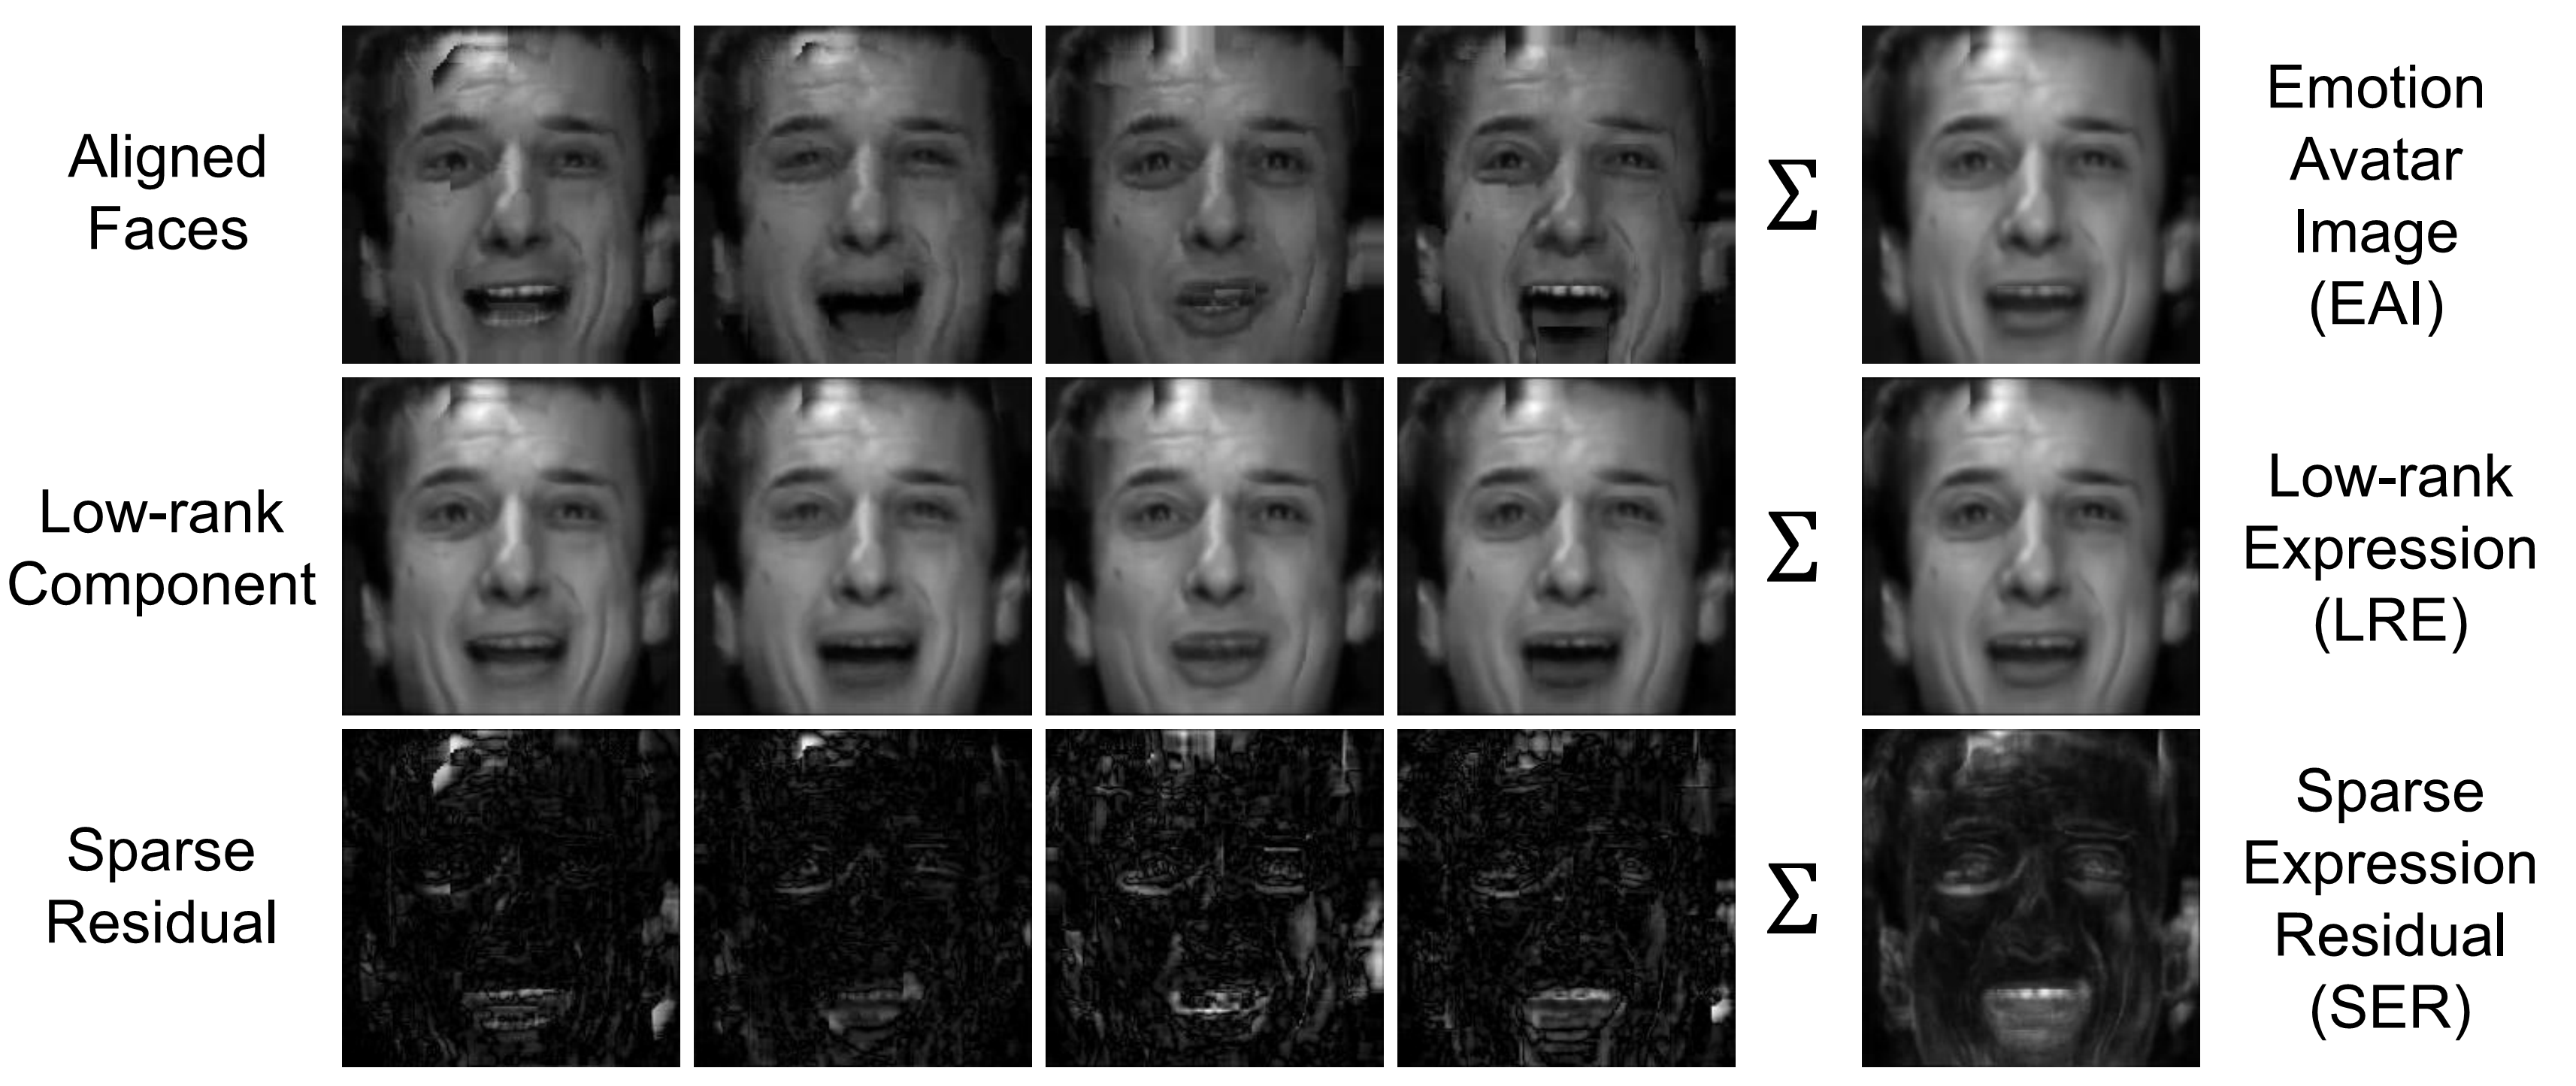
\includegraphics[width=\columnwidth]{pics/low_rank_sparse}
	\caption{The LRE and SER decomposition. A Low-rank component and a sparse residual component are jointly estimated and decomposed from a sequence of aligned expression images. Although individual frame differs from each other, the Mean LRE visually resembles the EAI representations.}
	\label{fig:low_rank_sparse}
\end{figure}


\subsection{Emotion Avatar Image (EAI) Revisited\label{sec:eai}}

EAI was proposed in~\cite{Yang_SMCB12} for the international competition on FERA Challenge~\cite{FERA11}. It is a robust image representation that summarizes facial expression videos and generalizes well for person-independent expression recognition. The EAIs are iteratively generated along with the Avatar Reference (AR) representation, which is canonical representation that captures the appearance of the entire dataset. The generalization of AR is also demonstrated in~\cite{Yang_SMCB12} such that the recognition performance is not degraded when AR is computed using contemporary datasets. As shown from row 1 of Fig.~\ref{fig:low_rank_sparse}, the EAI is computed from the mean of the aligned faces with respect to a certain level of AR (Level-1 in this case). It can be considered as a Maximum Likelihood estimate of the aligned sequences. 

On the other hand, the low-rank component and sparse residual of individual frame is recovered by Algorithm~\ref{alg}. As seen from row 2 of Fig.~\ref{fig:low_rank_sparse}, the low-rank components are jointly estimated from all frames of an sequence. Although individual frame appears to be different of each frame and its corresponding low-rank component, the maximum likelihood estimates of aligned faces (EAI) and their mean LRE resemble each other visually (last column of Fig.~\ref{fig:low_rank_sparse}). More sample visualizations are shown in Fig.~\ref{fig:eai_lre_compare} for various sequences. 


\begin{figure}[htbp]
	\centering
		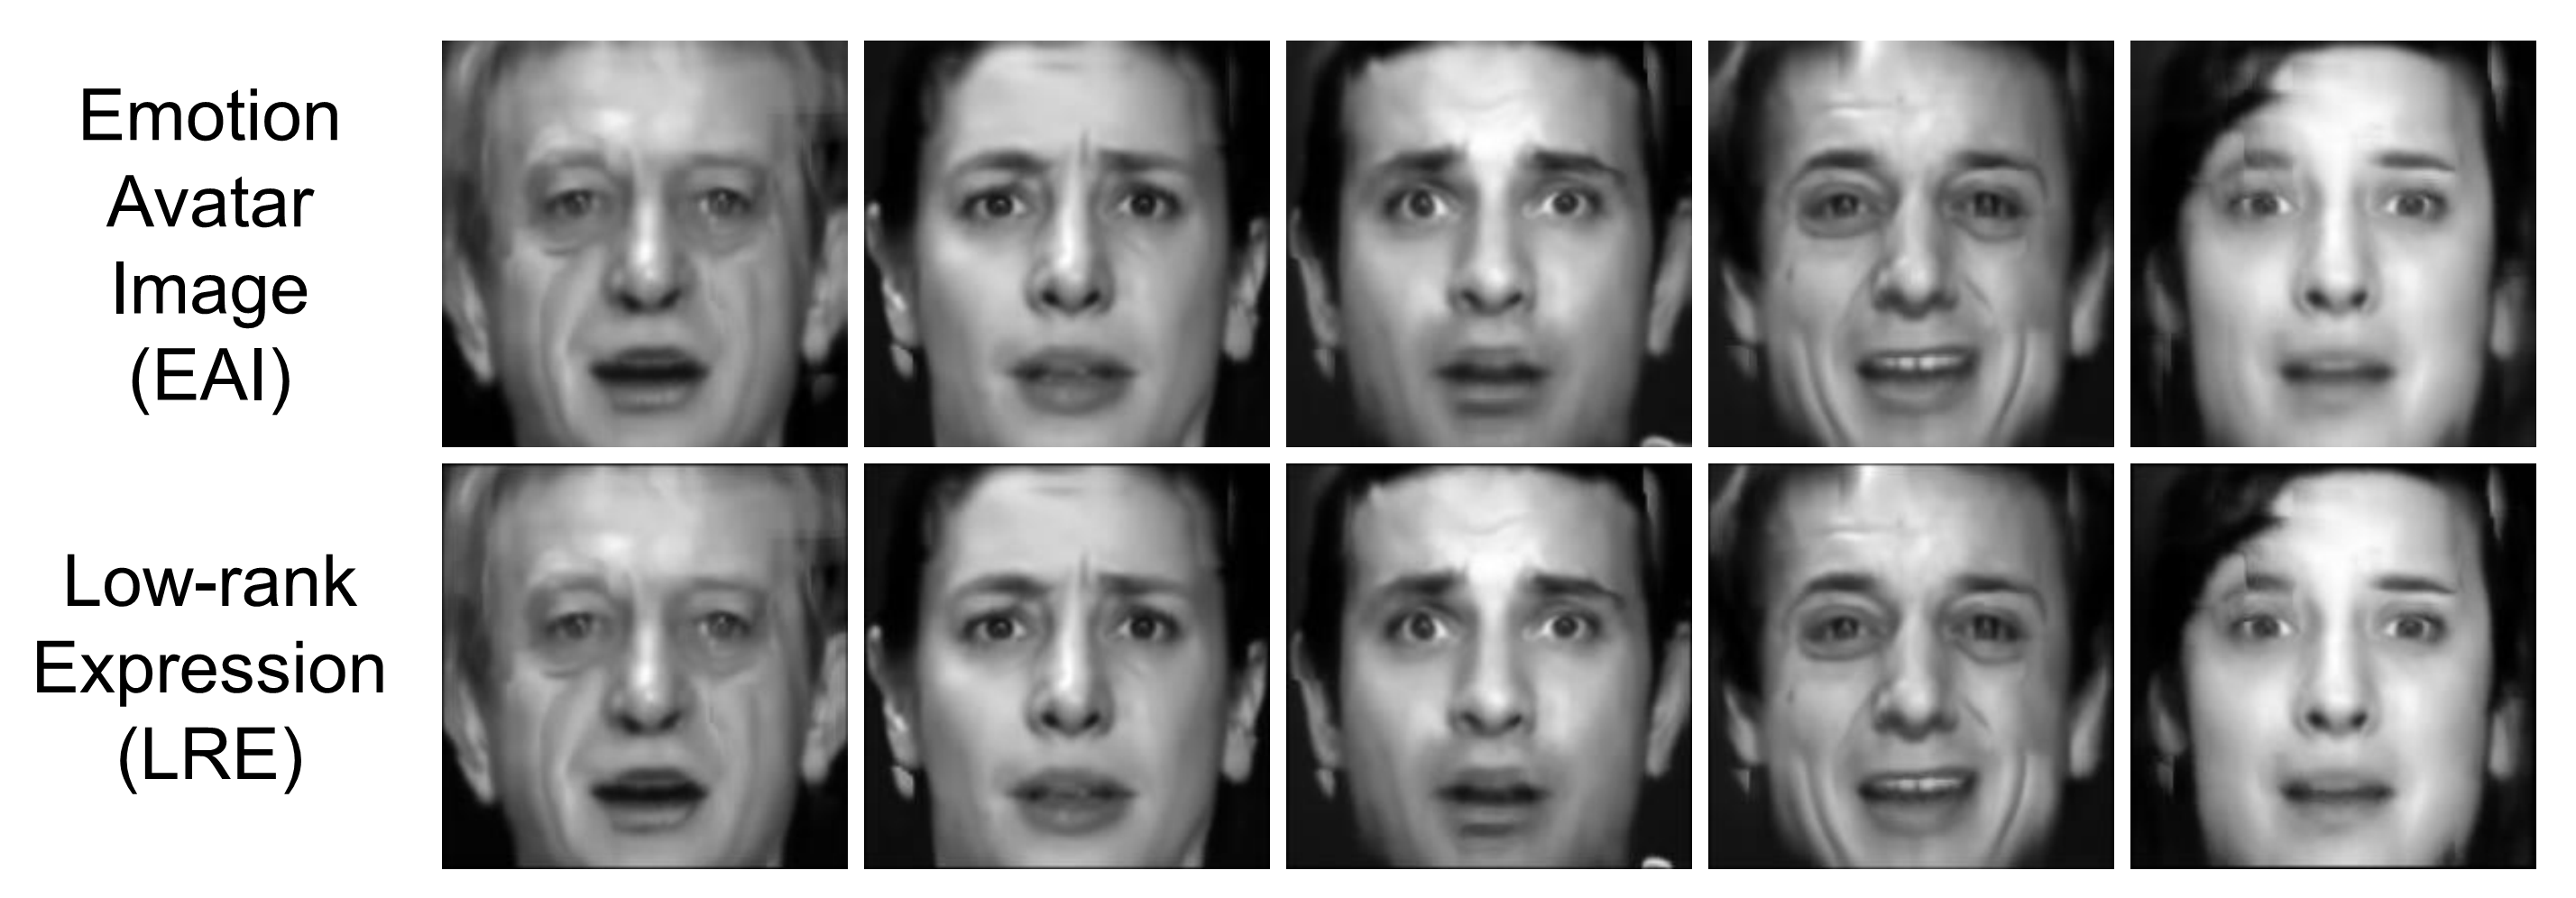
\includegraphics[width=\columnwidth]{pics/eai_lre_compare.png}
	\caption{The comparison of Low-rank Expressions (LRE) and Emotion Avatar Images (EAI). Although generated from different approaches, their appearances resemble each other at pixel level.}
	\label{fig:eai_lre_compare}
\end{figure}

As mentioned earlier, the expression appearance captured by the LRE reveals the underlining expression. For example, the expression \textit{Happiness} can be inferred from the LRE in Fig.~\ref{fig:low_rank_sparse} based on its lip corner expansion and cheek raise. However, LRE discards the expression dynamics of every individual. Fortunately, the sparse residual recovers the deviation of an aligned face from a low-rank expression frame. Sparse residual models the subtle muscle motion of each particular frame from the underlining expression. 

\begin{figure*}[htbp]
\centering{
        \subfigure[The Low-rank Expression (LRE) representations]{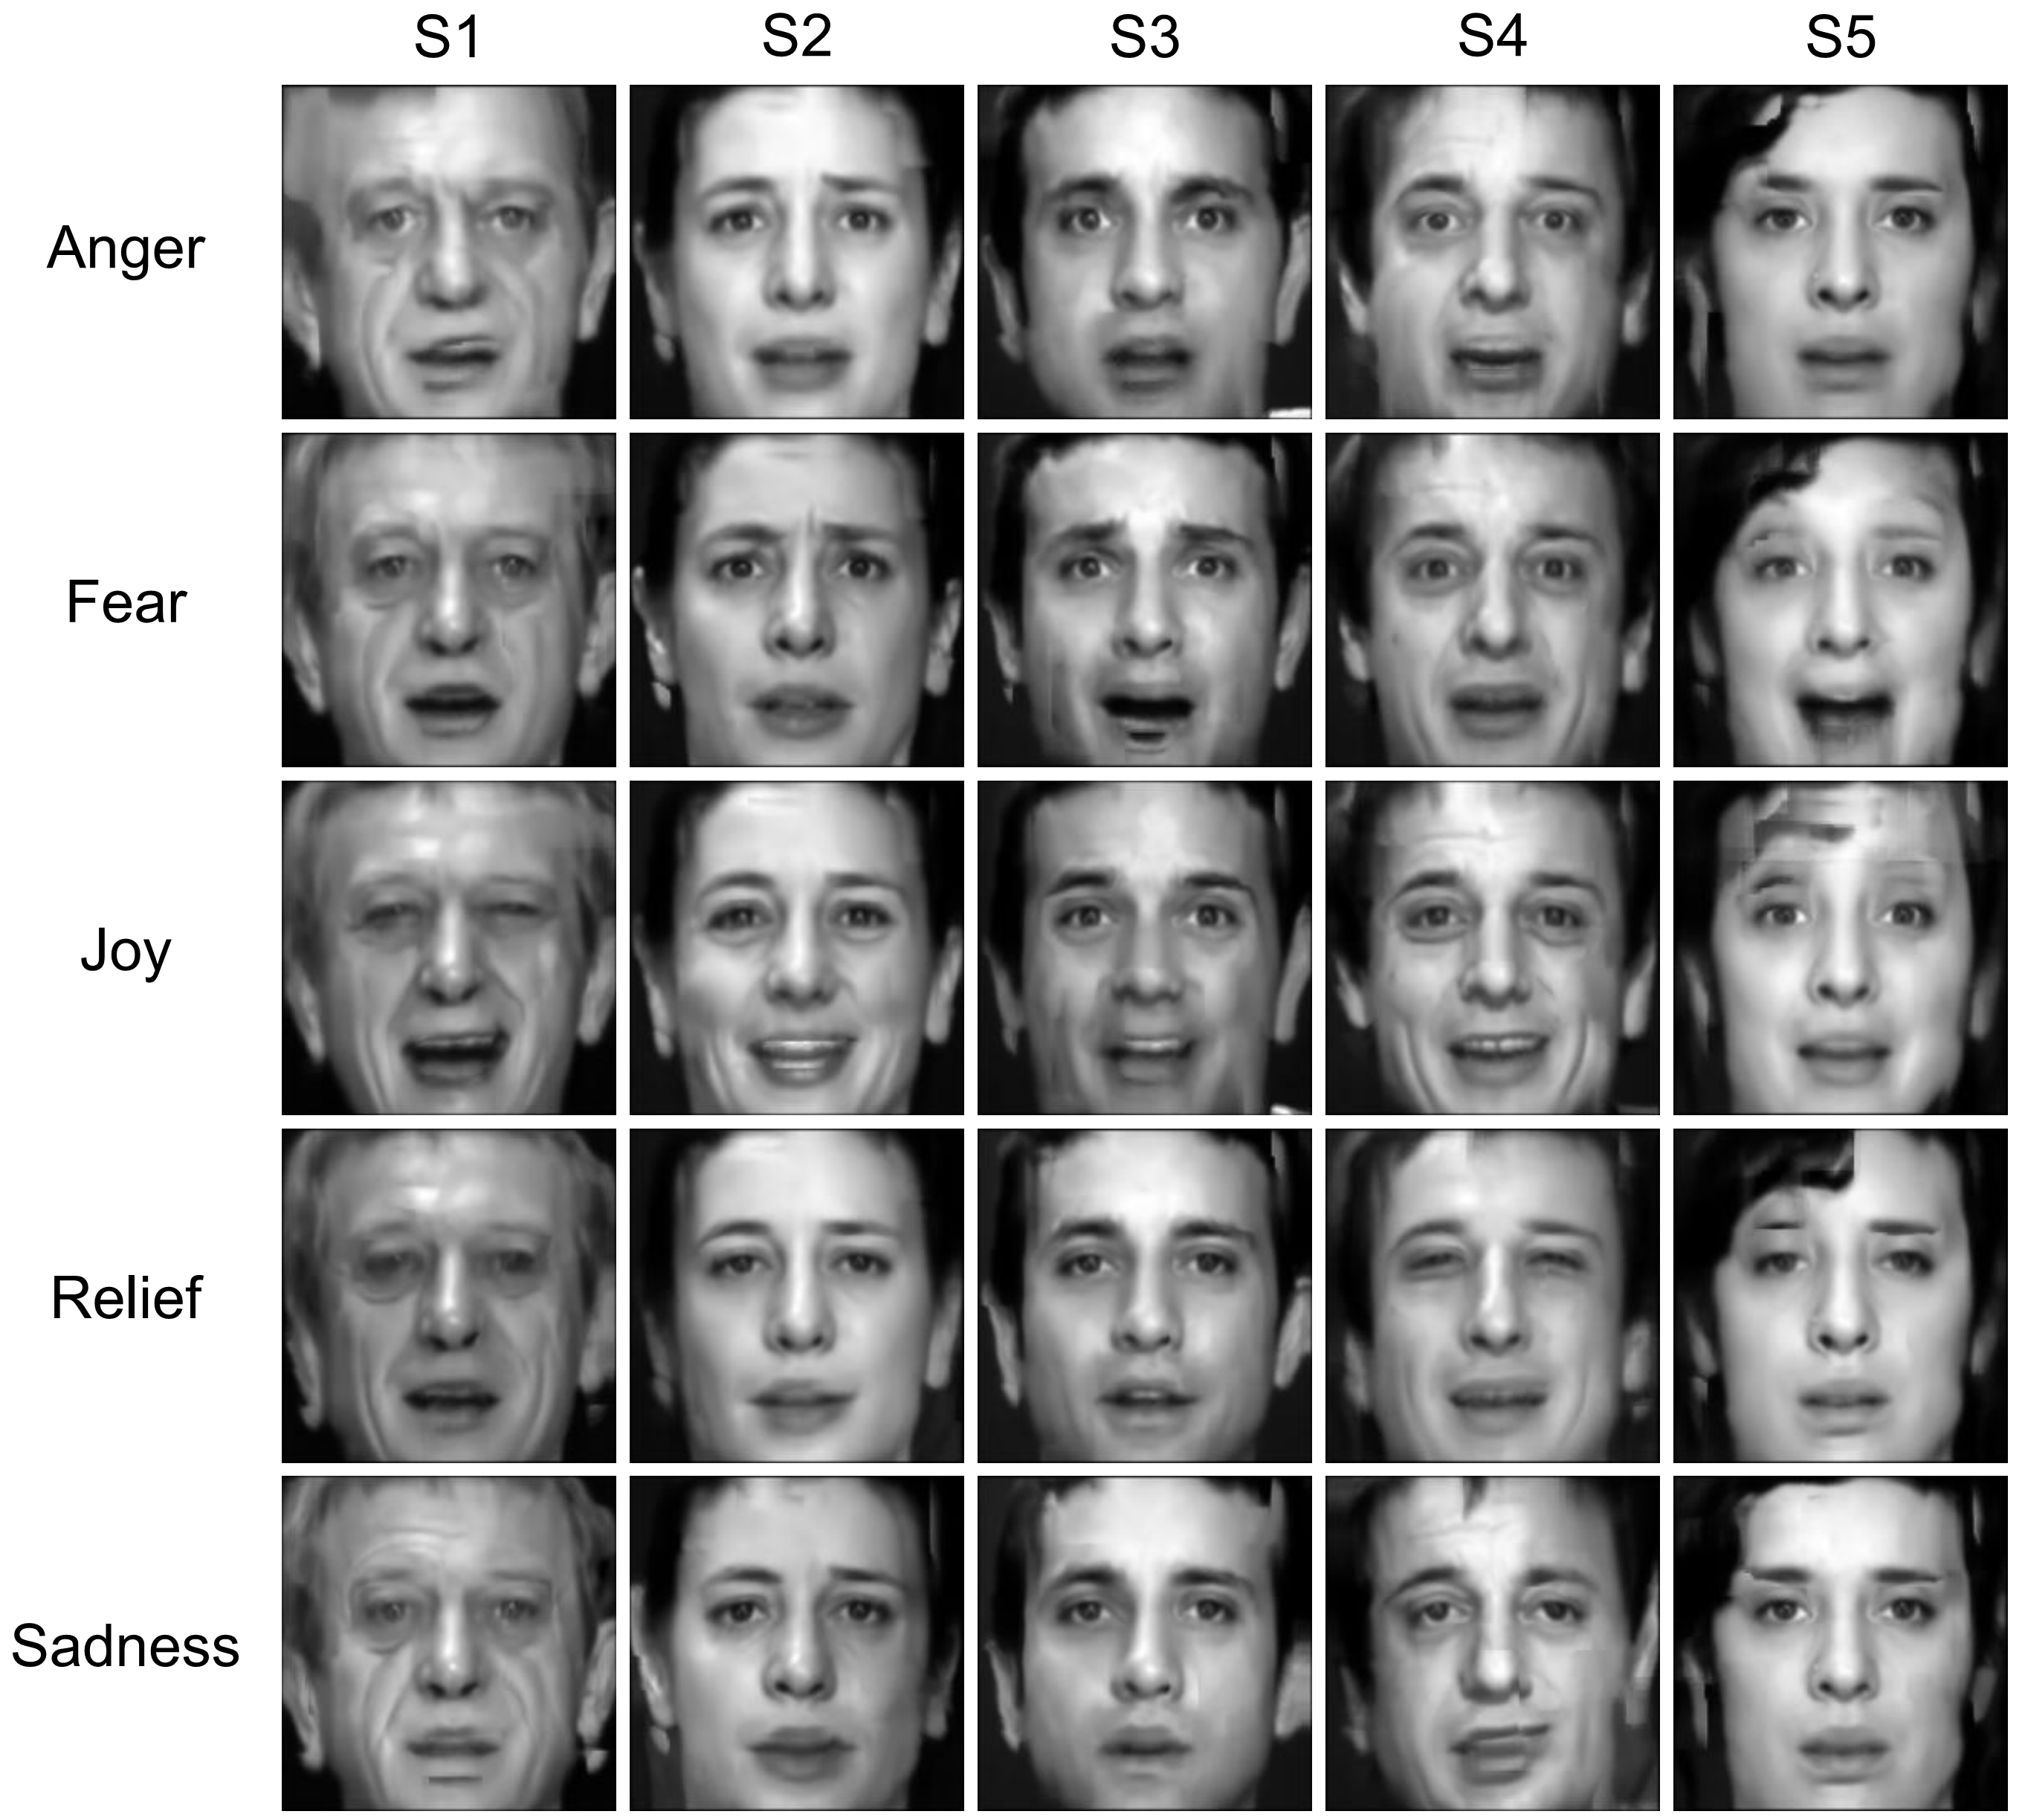
\includegraphics[width=0.45\linewidth]{pics/lre_vs_id.png}\label{fig:lre_vs_id}}
        \subfigure[The Sparse Residual Expression (SRE) representations]{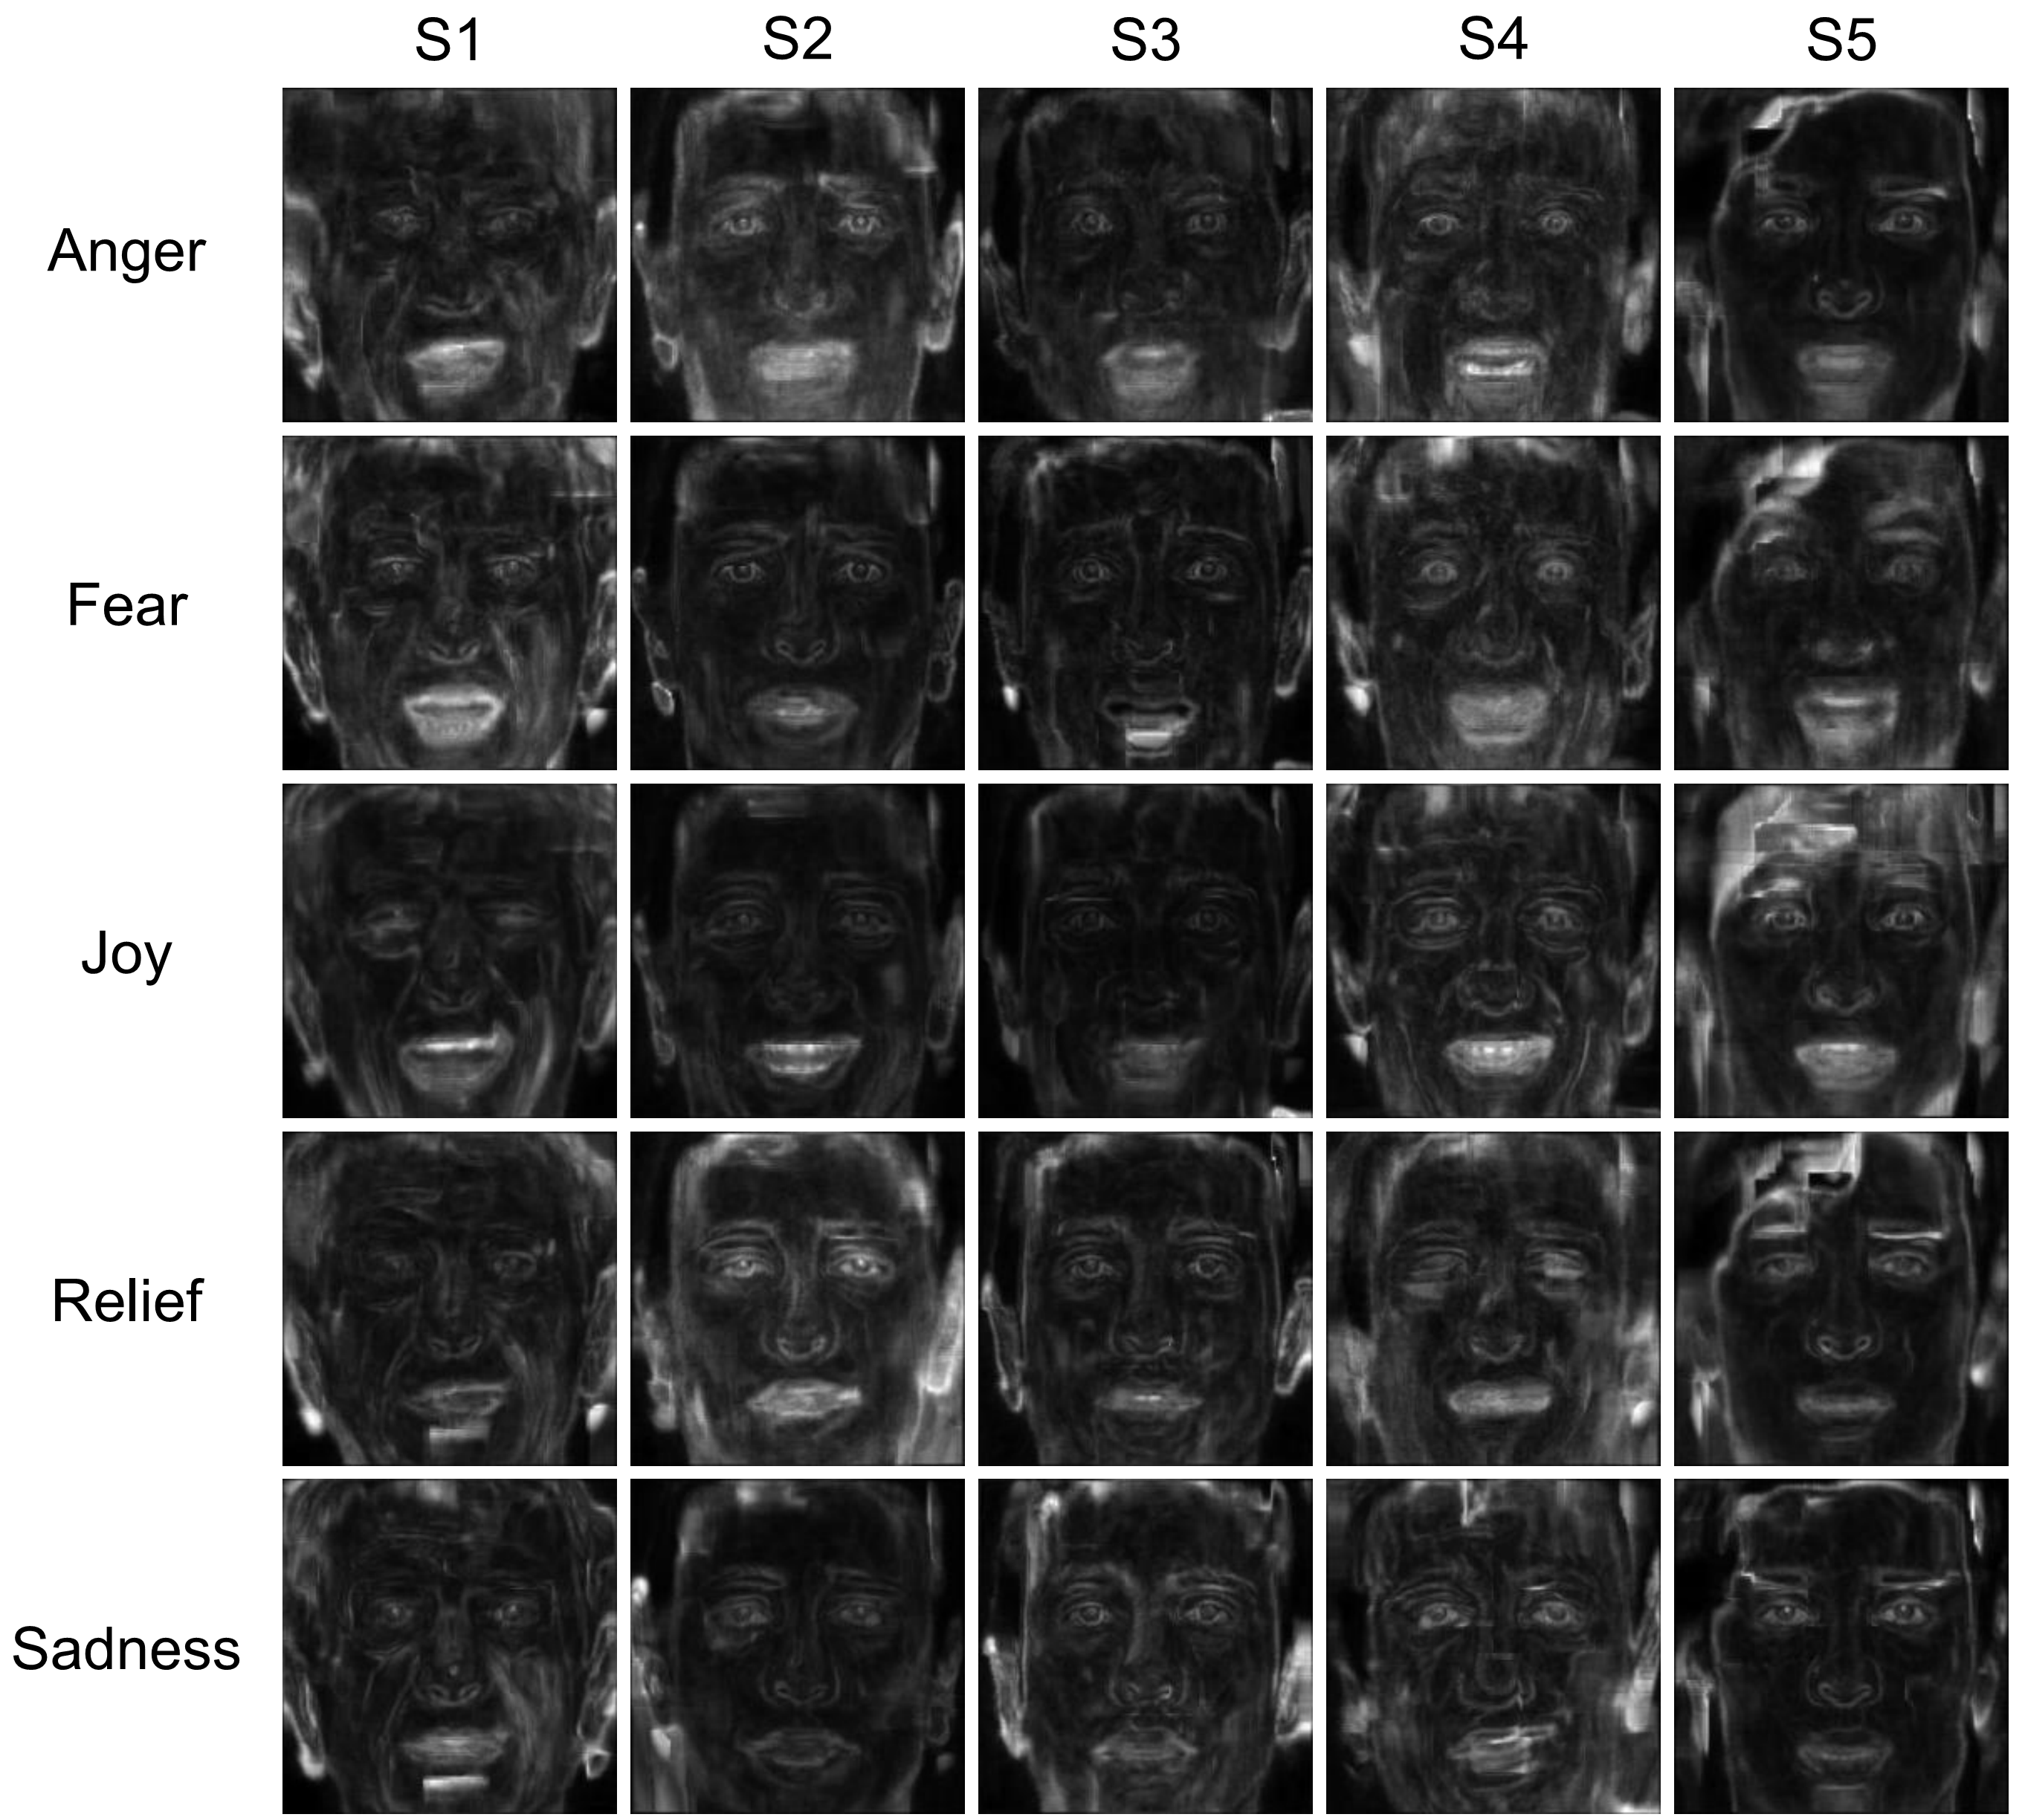
\includegraphics[width=0.45\linewidth]{pics/ser_vs_id.png}\label{fig:ser_vs_id}}
}
\caption{\label{fig:rep_vs_id} The sparse decomposition of facial expression sequence. Each grid is a image representation of a video sequence. Fig.~\ref{fig:lre_vs_id} shows the LRE representation and the corresponding grid in Fig.~\ref{fig:ser_vs_id} illustrates the SRE representation of the same expression sequence.}
\end{figure*}

\section{Experimental Results\label{sec:exp}}

We conduct experiments on the \textit{uncontrolled} benchmark, FERA-GEMEP dataset~\cite{FERA_data}. Qualitative results are first provided to visually demonstrate the validity of our method. The quantitative results then show that our method not only outperform the state-of-the-art approaches, but also has the potential of improvement given more data. We also provided results on the \textit{controlled} benchmark, CK+ dataset~\cite{CKplus}, for the completeness of the experiment.

\subsection{Experimental Setup}

In this work, the faces are first detected using the successful Viola-Jones face detector~\cite{Viola_IJCV04}. We then follow the standard image pre-processing steps in the literature~\cite{Valstar12}\cite{Yang_SMCB12} for a better and fair comparison. The detected face images are resized to $200\times200$ pixels, and then divided into blocks of size $20\times20$. Texture features are extracted at each local block and then concatenated to form a final feature vector for classification. The feature extraction is conducted on both LRE and SER modalities, respectively. To prevent over-fitting, Principal Component Analysis (PCA) is carried out and the space with $99\%$ of the variation is used for dimension reduction. Finally, Support Vector Machine (SVM)~\cite{libsvm} with linear kernel is used for our multi-class classification. The results of each modality and their combinations are all reported in the paper. 

\textbf{Static Feature:} various texture feature descriptors such as LBP and LPQ filters are used for feature extraction. To characterize the entire sequence using static feature, there are two strategies in general. First, one can extract features from individual frames and train a frame-based classifier. A final decision can be fused at the decision level by majority voting. Second, the feature extraction and classification can be conducted on the mean representation of the entire sequence. We have tested both strategies and found superior performance and faster processing speed for the latter strategy in general. Besides, this strategy is also used in~\cite{Yang_SMCB12}. Thus, we only report the results on the mean representation for the static feature extraction in this paper. 
\begin{enumerate}
\item Local Binary Pattern (LBP): LBP uses the local contrast statistics to characterize the image texture. In this work, we use the uniform LBP operator~\cite{Ojala_PAMI02} that generates 59 basic patterns for a local patch. Thus, the total feature dimension is $59\times 10\times 10=5900$. 
\item Local Phase Quantization (LPQ): proposed by Ojansivu \textit{et al.} in~\cite{LPQ}, LPQ descriptor is insensitive to image blur. The spatial blurring is modeled by the multiplication of the original image and a point spread function (PSF) in frequency domain. The key observation is that, when the PSF is centrally symmetric, the phase of the original image is invariant. The feature size for each patch is $256$, yielding a feature dimension of $25600$ in general. 
\end{enumerate}

\textbf{Dynamic Feature:} the LBP and LPQ can be extended to the temporal domain, capturing the dynamics of the texture. We consider two important variants, namely TOP-LBP and TOP-LPQ for dynamic feature extraction.
\begin{enumerate}
\item Three Orthogonal Planes LBP (TOP-LBP): the key idea of this dynamic histogram approach is to extend XY 2-D plane to three orthogonal directions, namely XY, XT, and YT, where the letter ``\textbf{T}'' denotes the temporal axis. The pattern co-occurrences of each plane are computed by their corresponding histograms; all histograms are then stacked to a single feature vector. This enlarges the feature dimension by a multiple of $3$. We uses a similar region segmentation as the aforementioned static feature and the total feature dimension is $3\times 5900=17700$ for TOP-LBP.

\item Three Orthogonal Planes LPQ (TOP-LPQ): a similar dynamic texture strategy can be applied to the LPQ extractor, resulting in a total feature dimension of $3\times 25600=76800$.  
\end{enumerate} 

In the following sections, we will report results of various combinations of static and dynamic features on both LRE and SER representations. 

\subsection{Uncontrolled Data: FERA-GEMEP Dataset}

The FERA-GEMEP~\cite{FERA_data} is an uncontrolled facial expression dataset, \textit{i.e.}, in the process of data collection, subjects are asked to convey one of the following five emotions at a time: \textit{Anger}, \textit{Fear}, \textit{Joy}, \textit{Relief}, \textit{Sadness}, without any control of their head or body movement. Each video segment contains one subject displaying expressions that corresponds to one emotion. The average video length is about 2 seconds with 30 fps frame rate. Most subjects are uttering some meaningless phrases while displaying expressions, and there are 3 to 5 videos for each subject with the same emotion. All experiments in this paper are designed to be \textit{person-independent} (\textit{i.e.} no test subject is in the training data), the performance of which is of the most interest because it shows the generalization ability of the algorithm. 


The FERA challenge consists of a training and a test set. There are 7 subjects (3 males and 4 females) in the training set, and 6 subjects (3 males and 4 females) in the test set, 3 of which appears in training. The facial expression videos of both sets are provided, while only the ground truth label for the training set is available. Fig.~\ref{fig:rep_vs_id} provides a visualization of the mean LRE and SRE representations of sample expression videos of various subjects for all emotion categories in the FERA training set. The participants can use other publicly available data in addition to FERA training set for training. The predictions on the test set are submitted to the FERA organizer for an independent evaluation. Table~\ref{table:fera_team} shows the challenge participants\footnote{\label{teams}Teams are ranked based on the FERA Challenge person-independent test. \textbf{UCR}: University of California at Riverside; \textbf{UCSD-CERT}: University of California at San Diego; \textbf{UIUC-UMC}: University of Illinois at Urbana-Champaign; University of Missouri; \textbf{KIT}: Karlsruhe Institute of Technology; \textbf{ANU}: Australian National University; \textbf{NUS}: National University of Singapore; \textbf{QUT-CMU}: Queensland University of Technology; Carnegie Mellon University; \textbf{UCL}: University College London; \textbf{UMont.}: University of Montreal;  \textbf{MIT-Cambridge}: Massachusetts Institute of Technology; University of Cambridge.} and the corresponding person-independent test results. 

Since the ground truth label is only available for the FERA training set, we evaluate our algorithm using this set. We carried out leave-one-subject-out cross validation using both static and dynamic features extracted from the LREs and SREs individually as well as their combinations, the results of which from LBP and LPQ variants are shown in Table~\ref{table:comp_lbp} and Table~\ref{table:comp_lpq}, respectively. The symbol ``-'' means a particular module is not used for feature extraction. In addition, we report the results of the best performing approach~\cite{Yang_SMCB12} in FERA challenge as a baseline comparison. We should stress that unlike most of the other methods which uses additional training data, only this work and~\cite{Yang_SMCB12} solely uses the FERA training set. 

Several interesting findings can be observed from the results in both Table~\ref{table:comp_lbp} and Table~\ref{table:comp_lpq}. First, the performance using static features on LRE only is on par with the EAI representation in~\cite{Yang_SMCB12}, $0.68$ for LBP and $0.7$ for LPQ. This is congruent with our qualitative analysis in Section~\ref{sec:eai} such that EAI and mean LRE has very similar appearance. Second, when considering single module performance, LRE results are consistently higher than SER ones (for both static and dynamic feature using both LBP and LPQ), which means LREs are more discriminative than SERs. This shows that, if only single module is considered, global structure of a facial expression is more informative than its local muscle motion. Third, combining both module almost always improves the recognition performance. For example, in Table~\ref{table:comp_lpq}, single module performances for LRE and SER are $0.7$ and $0.62$, respectively. Combining both modules improves the performance to $0.75$, which demonstrates the information captured by both modules complement each other. It also shows facial expression sequence are more informative than static expression images by exploiting the local muscle motion. Fourth, incorporating dynamic features further improves the performance. The best performance is generated when dynamic features are extracted from both the LRE and SER modules (in Table~\ref{table:comp_lbp} and Table~\ref{table:comp_lpq}). This informs us that the person-independent modeling is an effective strategy that not only diminishes the person-specific information to alleviate over-fitting, but also provides a reasonable manner for dynamic feature extraction. 

The confusion matrix for the best-performance setting, \textit{i.e.}, LRE+SER with TOP-LPQ, is tabulated in Table.~\ref{table:mat_fera}. \textit{Anger} and \textit{Fear} are misclassified to each other more often because the global structure of these two expressions are more similar compared with other expressions. As seen in~\cite{Valstar12}, \textit{Fear} is indeed the most challenging case for the FERA-GEMEP dataset. However, incorporating local muscle dynamics helps better characterizing the \textit{Fear} expression. 

\begin{table}
\caption{The rank of person-independent test in FERA Challenge\label{table:fera_team}}
\centering
\begin{tabular}{ll}
\toprule
	Teams~\ref{teams} & Accuracy \\ \midrule
	UCR 								& 0.75 \\ 
	UCSD-CERT						& 0.71 \\ 
	UIUC-UMC						& 0.66 \\ 
	KIT									& 0.66 \\ 
	ANU									& 0.65 \\ 
	NUS									& 0.64 \\ 
	QUT-CMU							& 0.62 \\ 
	UCL									& 0.61 \\ 
	UMont								& 0.58 \\ 
	MIT-Cambridge				& 0.45 \\ 
	Baseline						& 0.44 \\
\bottomrule
\end{tabular}
\end{table}

%\begin{table}[htbp]
%\caption{The accuracy comparison of our approach to the best performance system in the FERA Challenge\label{table:comp}}
%\begin{center}
%\begin{tabular}{|c|c|c|c|c|c|}
%\toprule
	%Approach 									& TOP-LPQ	& TOP-LBP 	& LPQ 	& LBP 	& Gabor \\ \midrule
	%LRE+SER										& \textbf{0.78} 		& 0.72 	& 0.76 	&	0.73	& 0.68	\\
	%UCR	\cite{Yang_SMCB12}		& 0.70 		& 0.67 	& \textbf{0.71} 	& 0.68	& 0.66	\\ 
	%LRE												& \textbf{0.72} 		& 0.66 	& 0.70 	& 0.68	& 0.66	\\
	%SER												& \textbf{0.65} 		& 0.65 	& 0.62 	& 0.60	& 0.55	\\
%\bottomrule
%\end{tabular}
%\end{center}
%\end{table}


\begin{table}[!t]
\caption{Classification accuracy on FERA-GEMEP dataset using LBP features\label{table:comp_lbp}}
\centering
\scriptsize
\begin{tabular}{lll||lll}
\toprule
LRE & SER & Accuracy	& LRE	& SER	& Accuracy \\ \midrule 
LBP	& -		& 0.68	& - & LBP & 0.6 \\
TOP-LBP & - & 0.67 & - & TOP-LBP & 0.62 \\
LBP & LBP & 0.7 & LBP & TOP-LBP & 0.72 \\
TOP-LBP & LBP & 0.7 & TOP-LBP & TOP-LBP & \textbf{0.73} \\ \midrule
\multicolumn{2}{l}{UCR~\cite{Yang_SMCB12}: LBP} & 0.68 & \multicolumn{2}{l}{UCR~\cite{Yang_SMCB12}: TOP-LBP} & 0.69 \\
\bottomrule

\end{tabular}
\end{table}


\begin{table}[!t]
\caption{Classification accuracy on FERA-GEMEP dataset using LPQ features\label{table:comp_lpq}}
\centering
\scriptsize
\begin{tabular}{lll||lll}
\toprule
LRE & SER & Accuracy	& LRE	& SER	& Accuracy \\ \midrule 
LPQ	& -		& 0.7	& - & LPQ & 0.62 \\
TOP-LPQ & - & 0.72 & - & TOP-LPQ & 0.65 \\
LPQ & LPQ & 0.75 & LPQ & TOP-LPQ & 0.77 \\
TOP-LPQ & LPQ & 0.76 & TOP-LPQ & TOP-LPQ & \textbf{0.78} \\ \midrule
\multicolumn{2}{l}{UCR~\cite{Yang_SMCB12}: LPQ} & 0.7 & \multicolumn{2}{l}{UCR~\cite{Yang_SMCB12}: TOP-LPQ} & 0.73 \\
\bottomrule

\end{tabular}
\end{table}




\begin{table}[htbp]
\caption{confusion matrix for the FERA training dataset using LER+SER.
(An=Anger, Fe=Fear, Jo=Joy, Re=Relief, Sa=Sadness)}
\begin{center}
\label{table:mat_fera}
\begin{tabular}{c|c|ccccc}
\multicolumn{7}{c}{True Label} \\ \cline{2-7}
\multirow{7}{*}{\begin{sideways}Prediction\end{sideways}} && An & Fe & Jo & Re & Sa \\ \cline{2-7}
&An				&\textbf{62.1} &13.2  &4.8  &3.6  &   \\ \cline{2-2}
&Fe       &16.4  &\textbf{71.4}  &3.2   &1.8   & \\ \cline{2-2}
&Jo       &7.5  &5.5   &\textbf{85.5} &3.6  &    \\ \cline{2-2}
&Re       &5.8   &1.8   &4.8   &\textbf{78.4} &8.6    \\ \cline{2-2}
&Sa       &8.2   &8.1   &1.6  &12.5 &\textbf{91.4}  \\ \cline{2-2}\hline
\multicolumn{2}{c|}{Average rate} &\multicolumn{5}{c}{\textbf{77.8}} \\

\end{tabular}
\end{center}
\end{table}


To dig deeper to our approach, we carry out more diagnostic experiments and analysis. If mentioned otherwise, the following analyses all use this best-performing setting. 

\textbf{The effect of Training Size with a fixed subject pool: } We observe that the performance of the EAI approach (\textit{i.e.}, $0.7$ shown in Table~\ref{table:comp_lpq} is inferior than that in the FERA challenge~\cite{Yang_SMCB12} (\textit{i.e.}, $0.75$ shown in Table~\ref{table:fera_team}). We believe that this is due to a smaller training size from our person-independent experiment setting. For validation, we carried out a leave-one-subject-out cross validation with respect to different training sizes for various representations. For a specific size, we randomly select the training data according to person-independent constraint from the subject pool to train a classifier. This experiment is repeated for 10 times at each training size, and the average classification rate is reported in Fig.~\ref{fig:effect_training_size}. As seen in Fig.~\ref{fig:effect_training_size}, the classification rate steadily raises as the training size increases for all three curves. This informs us that given more training data for same training subject pool, the algorithm performance increases. Additionally, it is observed that the increase rate for LRE is boosted by SER, especially when training size becomes larger. This demonstrates that the SER indeed captures more discriminative facial muscle motion for expression recognition. In the meantime, the performance of LRE+SER is not saturated as the training size reaches the maximum (130 in this experiment), suggesting a potential for better performance given more data.


\begin{figure}[htbp]
	\centering
		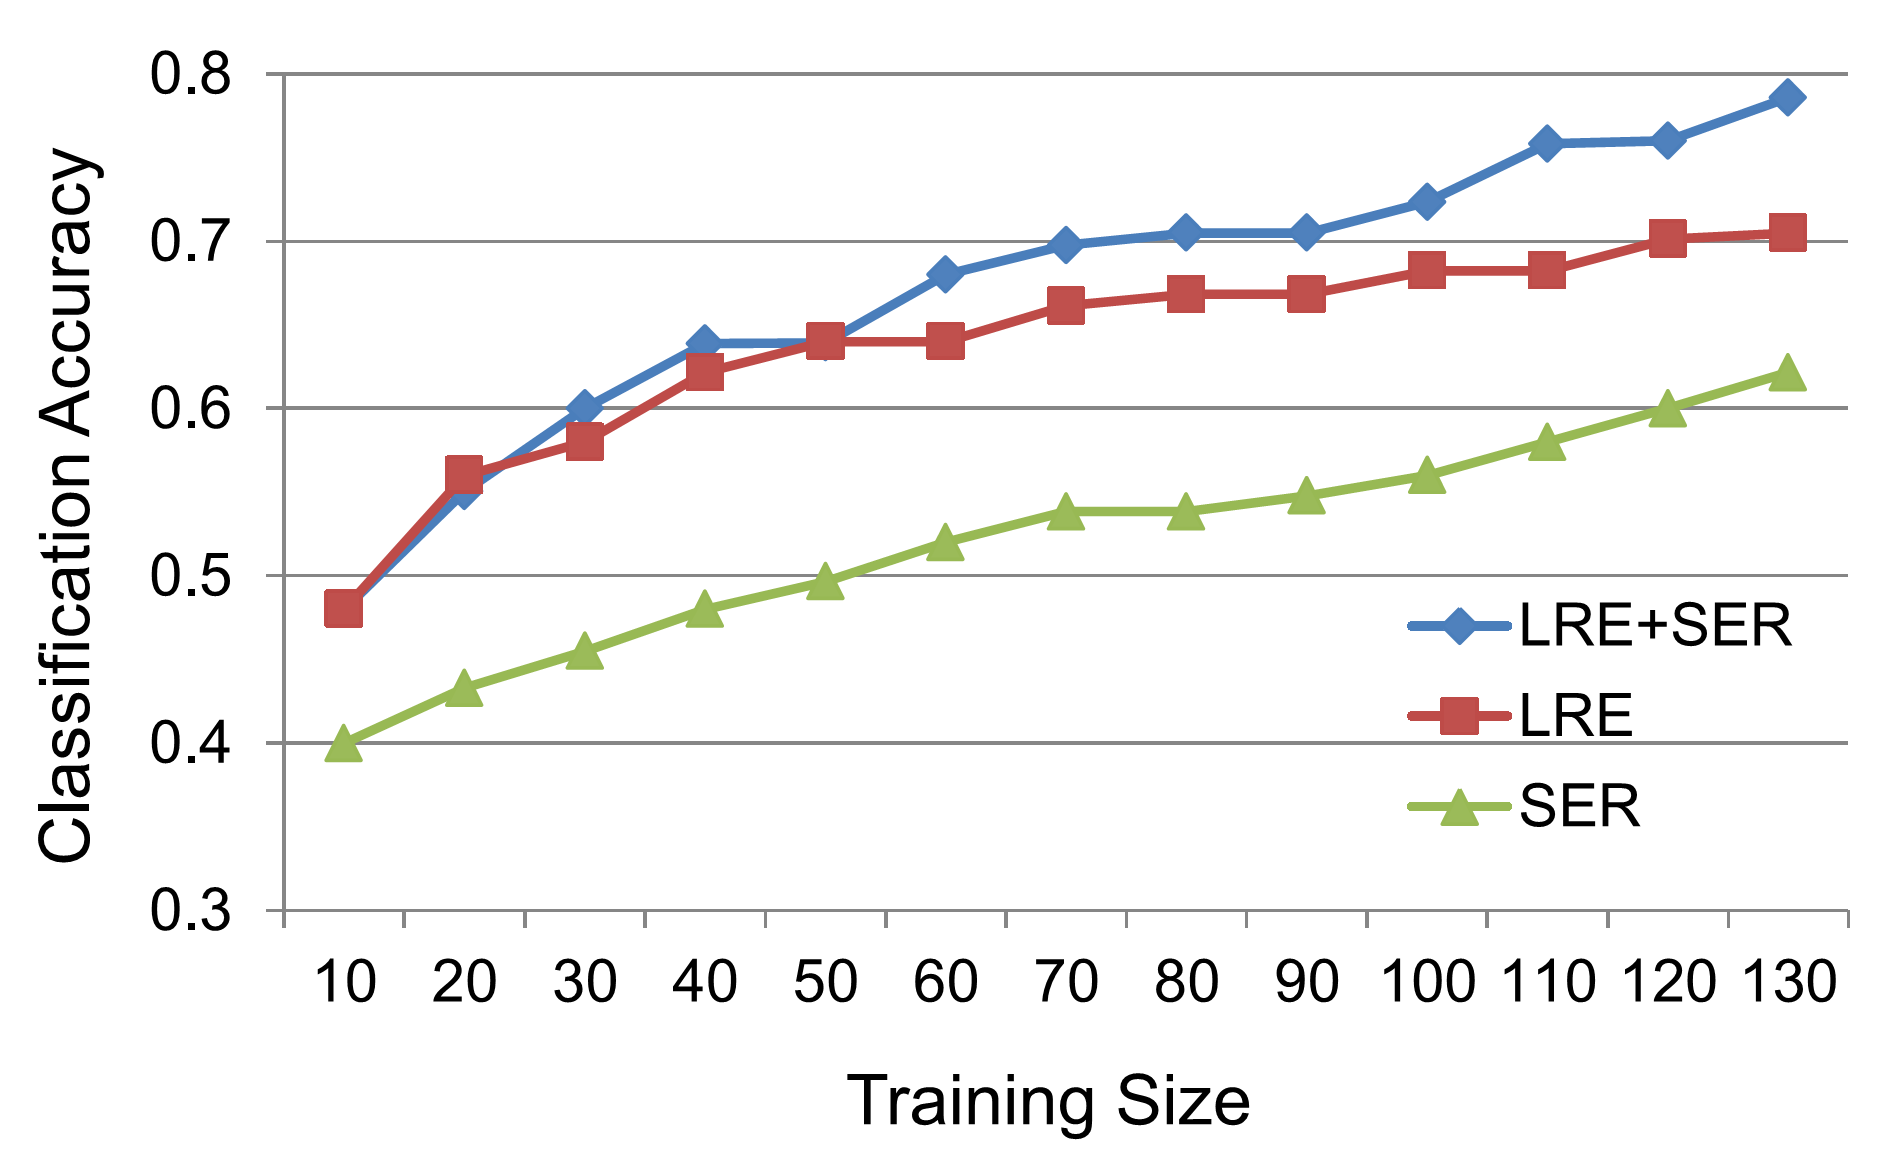
\includegraphics[width=.8\columnwidth]{pics/effect_training_size.png}
	\caption{The person-independent recognition accuracy trend with various training size. The feature in use is TOP-LPQ. The performance of LRE is spurred by the additional information captured in SER, and it has the potential for superior performance as the number of training increases.}
	\label{fig:effect_training_size}
\end{figure}

\textbf{The size of Subject Pool: } under a person-independent setting, it is also interesting to discover the impact of the number of subjects in training. Thus, for each leave-one-subject-out test using LRE+SER, we vary the number of subjects in training, $k$, from 1 to 6 (since there are 7 subjects in the dataset), and conduct the test for ${6 \choose k}$ times. For example, when 2 subjects are in the training, there can be ${6 \choose 2}=15$ possible combinations of subjects, we record the test results for all combinations. As illustrated in Fig.~\ref{fig:effect_people_num}, a boxplot shows an increasing trend for classification accuracy as the number of subjects in training increases. This shows that the performance is likely to be improved as the number of training subjects enlarges. Additionally, the decreasing variance of the classification accuracy can be observed from Fig.~\ref{fig:effect_people_num}, suggesting a more stable performance as the number of training subjects pool increases. 


\begin{figure}[htbp]
	\centering
		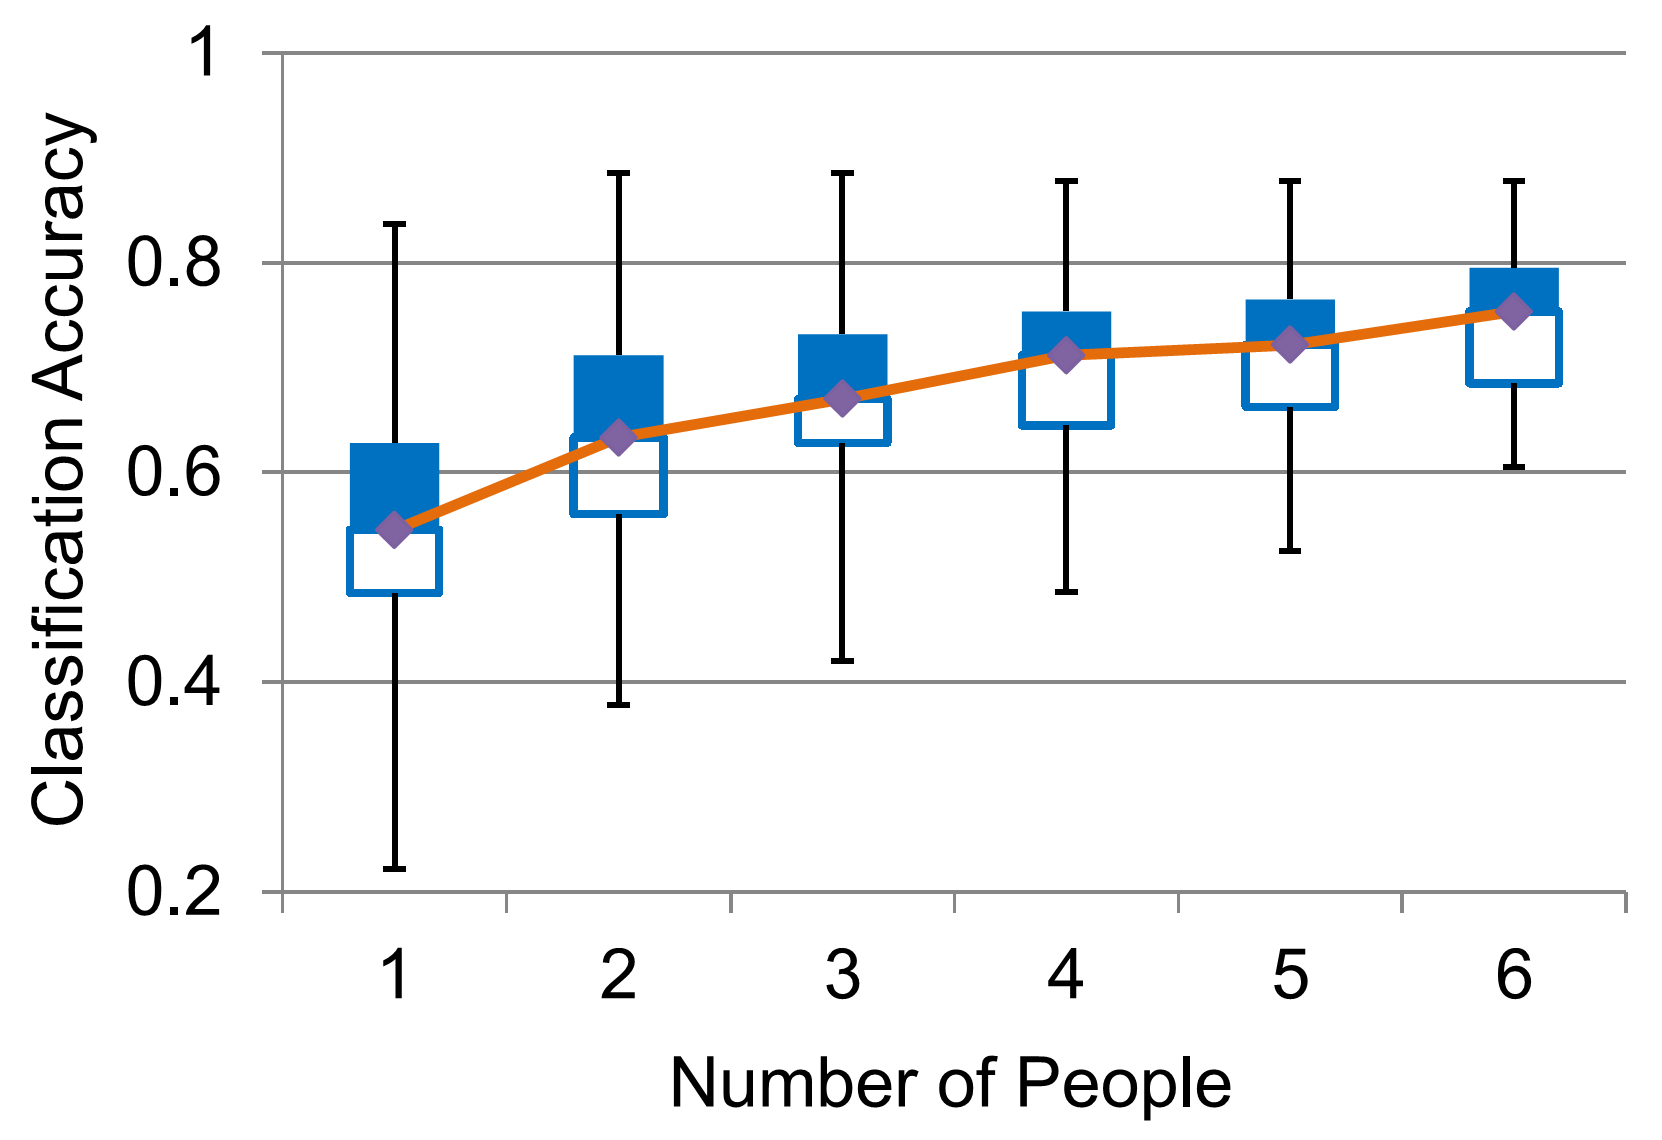
\includegraphics[width=.65\columnwidth]{pics/effect_people_num.png}
	\caption{The boxplot of person-independent recognition accuracy using LRE+SER and TOP-LPQ with various number of people in the training set. The mean performance at the second quartile are connected to illustrate the trend. In general, the performance increases and becomes more stable when the number of training subjects pool enlarges.}
	\label{fig:effect_people_num}
\end{figure}



\subsection{Controlled Data: CK+ dataset}

The Extended Cohn-Kanade dataset (CK+)~\cite{CKplus} is a facial expression dataset that has 7 categories of expressions, namely, \textit{Anger}, \textit{Contempt}, \textit{Disgust}, \textit{Fear}, \textit{Happy}, \textit{Sadness}, and \textit{Surprise}. This is a controlled dataset since the subjects controlled their head pose on purpose, and the expression displayed always follows the ``neutral-onset-apex" pattern. These conscious control may not only hide the true muscle contraction of an expression, but also changes the expression dynamics~\cite{Bartlett03}\cite{Ekman2005}. Although the philosophy of our algorithm is not designed for this fully controlled data, for the sake of completeness of a study, we also carry out person-independent tests and evaluate our LRE+SER representation together with the static LPQ feature descriptor on 316 sequences from 123 subjects in this dataset. The static LPQ is chosen for a better comparison with the literature. 

\begin{table}[htbp]
\caption{confusion matrix for CK+ dataset using LER+SER.
(An=Anger, Co=Contempt, Di=Disgust, Fe=Fear, Ha=Happy, Sa=Sadness, Su=Surprise)}
\begin{center}
\label{table:CK_result}
\begin{tabular}{c|c|ccccccc}

\multicolumn{9}{c}{True Label} \\ \cline{2-9}
\multirow{8}{*}{\begin{sideways}Prediction\end{sideways}} && An & Co & Di & Fe & Ha & Sa & Su \\ \cline{2-9}
&An          &\textbf{75} &22.2  &1.8  &8  &  &25.9 &  \\ \cline{2-2}
&Co       &2.3  &\textbf{72.2}  &   &   &  &3.7  &1.2 \\ \cline{2-2}
&Di        &4.5  &   &\textbf{94.6} &  &1.6 &3.7 &2.4  \\ \cline{2-2}
&Fe           &2.3   &   &   &\textbf{68} &  &3.7  &1.2  \\ \cline{2-2}
&Ha          &4.5   &   &1.8  &8 &\textbf{96.8} &  &  \\ \cline{2-2}
&Sa        &9.1  &  &  &4   &  &\textbf{48.1} & \\ \cline{2-2}
&Su       &2.3  &5.6 &1.8  &12 &1.6  &14.8 &\textbf{95.2} \\ \hline
\multicolumn{2}{c|}{Average rate} &\multicolumn{7}{c}{\textbf{85.1}} \\

\end{tabular}
\end{center}
\end{table}


As seen in Table~\ref{table:CK_result}, the LRE+SER representation achieves $85.1\%$ accuracy on average, outperforming $82.6\%$ by the EAI representation~\cite{Yang_SMCB12}. Once again, this demonstrates that the information captured by the SER improves the expression recognition accuracy. The algorithm~\cite{Zhao_PAMI07} using the same dynamic texture feature, LBP-TOP, has a better performance on CK+ dataset. We believe it is because the experiment in~\cite{Zhao_PAMI07} are designed as 10-fold cross validation. Although there is no subject that displays the same expression twice in CK+, this experiment setting does not strictly guarantee no test subject in training. On the contrary, our experimental design is strictly person-independent.

Besides, the CK+ data has only one or a few apex expression for each ``neutral-onset-apex" sequence. This unrealistic setting reduces the intensity of the expression captured by LREs, which appears to be more neutral compared with the mean LRE of FERA-GEMEP data. Fig.~\ref{fig:ck_eai} shows a visualization of mean LRE representations for sample sequences from the CK+ dataset. 

In addition, through a diagnostic experiment, we have found that the classification performance has a strong correlation with the training size for each class category, shown in Fig.~\ref{fig:fig_ck_size}. We plot the classification accuracy along with the training size for each category in Fig.~\ref{fig:fig_ck_size}. The categories such as Disgust, Happy, and Surprise, which have more data in training, have a much higher accuracy. This also shows the potential of improvement for our algorithm given more training sample for the under-performing categories. 

\begin{figure}[htbp]
	\centering
		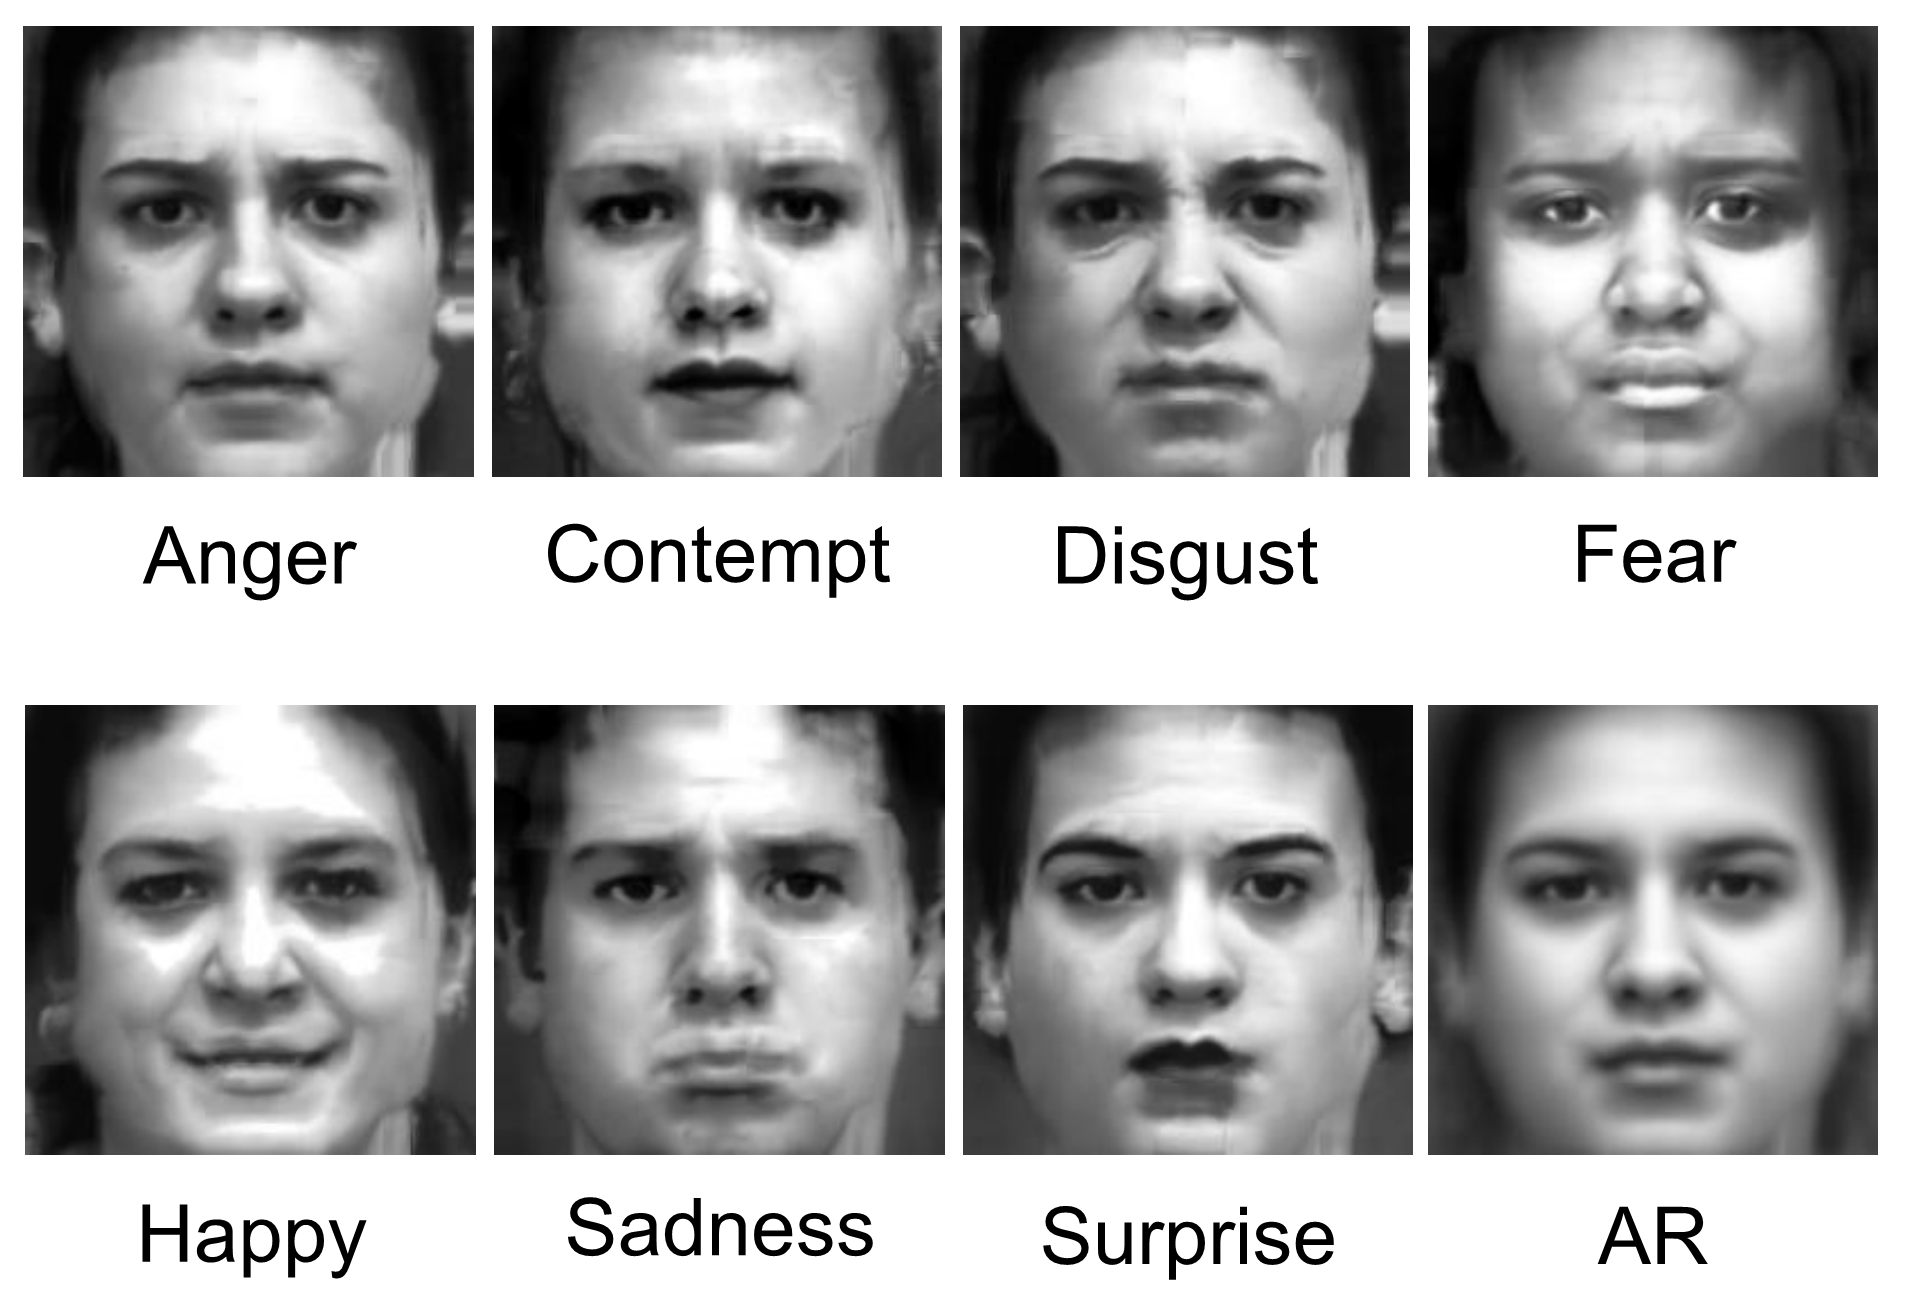
\includegraphics[width=.7\columnwidth]{pics/ck_eai.png}
	\caption{Sample mean LRE representations for the CK+ dataset. The lower right grid shows the Avatar Reference generated from~\cite{Yang_SMCB12}. Although the person-specific information is attenuated as the appearance of different subjects visually resemble each other, the discriminative expression information is hidden and difficult to be distinguished. In general, they appear to be more ``neutral'' compared with the mean LRE representations of sequences in FERA-GEMEP dataset in Fig.~\ref{fig:lre_vs_id}.}
	\label{fig:ck_eai}
\end{figure}

\begin{figure}[htbp]
	\centering
		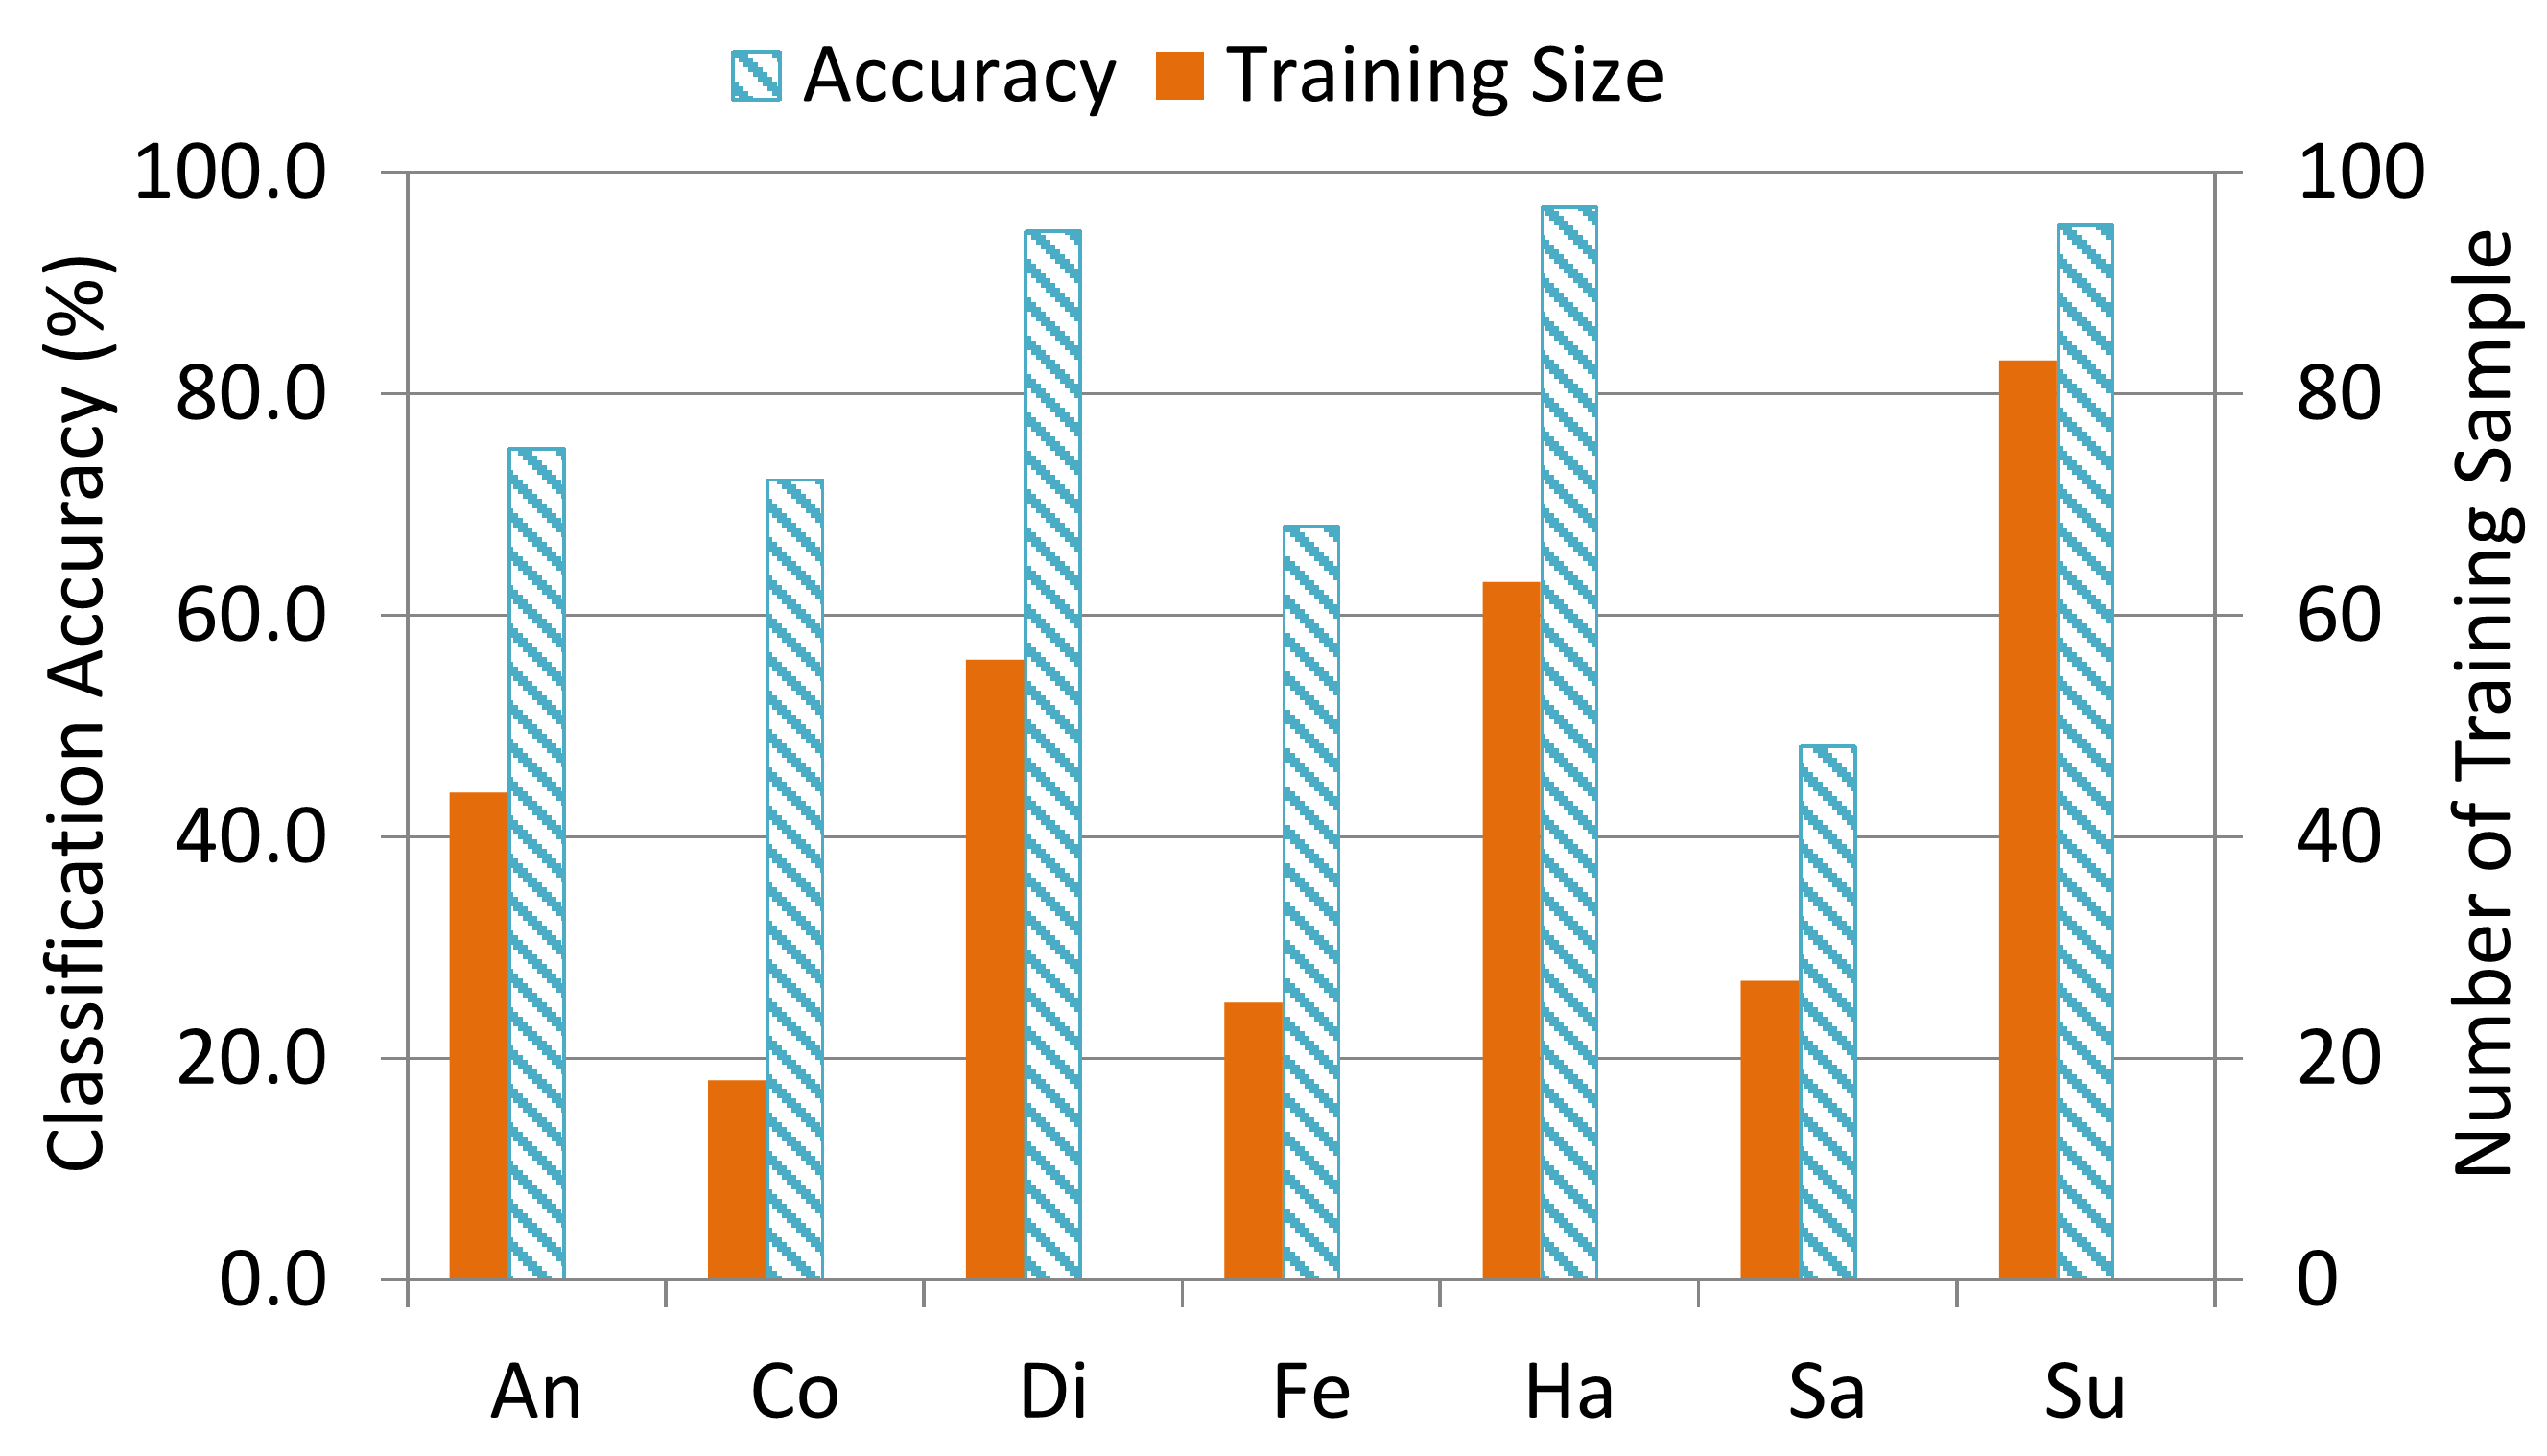
\includegraphics[width=.8\columnwidth]{pics/fig_ck_size.png}
	\caption{Relation between the classification accuracy and the training size for each expression category. The accuracy is generally higher for categories with more training data.}
	\label{fig:fig_ck_size}
\end{figure}



\section{Conclusions\label{sec:conclude}}
We have proposed a low-rank sparse recovery framework to effectively extract dynamic muscle motion for person-independent facial expression recognition. Our approach decomposes a facial expression sequence into two representations, namely the Low-rank Expression (LRE) and the Sparse Expression Residual (SER). The LRE recovers the underline expression appearance shared the entire expression sequence while SER captures the local muscle motion. The LRE and SER complement each other for a better expression recognition performance. In addition, our approach has the potential of improvement given more training samples and larger training subject instances. 


% Can use something like this to put references on a page
% by themselves when using endfloat and the captionsoff option.
\ifCLASSOPTIONcaptionsoff
  \newpage
\fi


\bibliographystyle{IEEEtran}
\bibliography{expression}





% that's all folks
\end{document}


